%
% Master thesis template for Ghent University (2021)
%
%
%  !!!!!!!!!!!!!!!!!!!!!!!!!!!!!!!!!!!!!!!!!!!!!!!!!!!!!!!!!!!!
%  !!  MAKE SURE TO SET lualatex OR xelatex AS LATEX ENGINE  !!
%  !!!!!!!!!!!!!!!!!!!!!!!!!!!!!!!!!!!!!!!!!!!!!!!!!!!!!!!!!!!!
%  !! For overleaf:                                          !!
%  !!     1. click gear icon in top right                    !!
%  !!     2. select `lualatex` in "latex engine"             !!
%  !!     3. click "save project settings"                   !!
%  !!                                                        !!
%  !!!!!!!!!!!!!!!!!!!!!!!!!!!!!!!!!!!!!!!!!!!!!!!!!!!!!!!!!!!!
%
%
%  History
%    2014         Doctoral Thesis of Bruno Volckaert
%    2017         Adapted to master thesis by Jerico Moeyersons
%    2018         Cleanup by Merlijn Sebrechts
%    2021         Update by Marleen Denert and Merlijn Sebrechts with feedback from Leen Pollefliet
%
%  Latest version
%    https://github.com/galgalesh/masterproef-template
%
\documentclass[11pt,a4paper,openany]{book}
\usepackage[a4paper,includeheadfoot,margin=2.50cm]{geometry}

\setlength{\parindent}{0cm}           % indent of the first sentence of a paragraph
\setlength{\parskip}{1em}             % space between paragraphs

\renewcommand{\baselinestretch}{1.2}  % stretch horizontal space between everything

\usepackage[hyphens]{url} % Break line on hyphens in long urls
\usepackage{graphicx}
\graphicspath{{images/}}
\usepackage{pdfpages}
\usepackage{enumitem}
\usepackage{float}
\usepackage{caption}
\usepackage{subcaption}
\usepackage[toc,page]{appendix}
\usepackage{fontspec}
\usepackage[T1]{fontenc}

% Don't indent table of contents, list of figures, and list of tables
\usepackage{tocloft}
\setlength{\cftsecindent}{0pt}    % Remove indent for \section
\setlength{\cftsubsecindent}{0pt} % Remove indent for \subsection
\setlength{\cftfigindent}{0pt}    % remove indentation from figures in lof
\setlength{\cfttabindent}{0pt}    % remove indentation from tables in lot

% To generate fake lorem ipsum text
\usepackage{lipsum}



%
% UGent style guide
%
\setmainfont[
	Path=fonts/,
	BoldFont      =UGentPannoText-SemiBold.ttf,
	ItalicFont    =UGentPannoText-Normal.ttf,
	ItalicFeatures={FakeSlant=0.3},
	BoldItalicFont=UGentPannoText-SemiBold.ttf,
    BoldItalicFeatures={FakeSlant=0.3},
]{UGentPannoText-Normal.ttf}
\urlstyle{same} % Also use the default font for URLs


% If you want left justified text, uncomment the line below.
%\usepackage[document]{ragged2e} % Left justify all text

% Style Chapter titles so they have the chapter number in grey.
\usepackage{color}
\definecolor{chaptergrey}{rgb}{0.5,0.5,0.5}
\usepackage[explicit, pagestyles]{titlesec}
\titleformat{\chapter}[display]{\bfseries}{\color{chaptergrey}\fontfamily{pbk}\fontsize{80pt}{100pt}\selectfont\thechapter}{0pt}{\Huge #1}
\titlespacing*{\chapter}{0pt}{-80pt}{30pt}


% Header showing chapter number and title and footer showing page number
\newpagestyle{fancy}{%
  \sethead{} % left
          {} % center
          {\Large\thechapter~~\chaptertitle} %right
  \setfoot{} % left
          {\thepage} % center
          {} %right
  \setheadrule{0pt}
}
\pagestyle{fancy}

% Header showing chapter title and footer showing page number
\newpagestyle{numberless}{%
  \sethead{} % left
          {} % center
          {\Large\chaptertitle} %right
  \setfoot{} % left
          {\thepage} % center
          {} %right
  \setheadrule{0pt}
}

\usepackage{minted}                                    % for modern code highlighting
\newenvironment{code}{\captionsetup{type=listing}}{}   % To get multiline code fragments working: https://tex.stackexchange.com/a/53540/72273

\PassOptionsToPackage{hyphens}{url}
\usepackage{hyperref}
\usepackage{url}

\usepackage[numbers]{natbib}       % For bibliography; use numeric citations
\bibliographystyle{IEEEtran}
\usepackage[nottoc]{tocbibind}     % Put Bibliography in ToC

%
% Defines \checkmark to draw a checkmark
%
\usepackage{tikz}
\def\checkmark{\tikz\fill[scale=0.4](0,.35) -- (.25,0) -- (1,.7) -- (.25,.15) -- cycle;}

%
% For tables
%
\usepackage{booktabs}
\usepackage{array}
\usepackage{ragged2e}  % for '\RaggedRight' macro (allows hyphenation)
\newcolumntype{L}[1]{>{\raggedright\let\newline\\\arraybackslash\hspace{0pt}}m{#1}}
\newcolumntype{C}[1]{>{\centering\let\newline\\\arraybackslash\hspace{0pt}}m{#1}}
\newcolumntype{R}[1]{>{\raggedleft\let\newline\\\arraybackslash\hspace{0pt}}m{#1}}

%
% Support for splitting Dutch words correctly
%
\usepackage{polyglossia}
\setdefaultlanguage[babelshorthands=true]{dutch}

% Manually specify additional hypnations for words
%
% Translated strings. If these aren't set, the English words are used.
%
\addto\captionsenglish{%
  \renewcommand{\contentsname}%
    {Inhoudsopgave}%
}


\renewcommand\appendixtocname{Bijlagen}
\renewcommand\appendixpagename{Bijlagen}
\renewcommand{\listoflistingscaption}{Lijst van listings}

%
% Set the title and your name
%
\title{Using GANs to optimize Pose Estimation on Art Collections}
\author{Tristan Verheecke}

%
%  END OF HEADER
%  The actual latex document content starts here.
%
\begin{document}
%download het voorblad van plato
\frontmatter

\includepdf{voorblad.pdf}

% White page
\newpage\thispagestyle{empty}\mbox{}
\mainmatter
% Word of thanks
\chapter*{Preface}

I've been interested in Art my entire life. In fact, I've a degree in the Fine Arts from LUCA School of Arts.
There, I was known for my technological ability and one of my professors at the time asked me why I didn't do anything with that in my artworks.
That remark has since stuck with me and was part of my motivation to apply for readmission for my Master of Science.
With all the advancements in AI, I started thinking more and more about doing work with that.
Like Matisse and Turner, I'm not satisfied with the tools available but want to create my own.

It was therefor to my delight that I was able to work on this thesis which has provided me the opportunity to acquire more insight in the subject.
I would like to thank my supervisors Dieter De Witte and Steven Verstockt for this wonderful opportunity,
and my counsellor Kenzo Milleville for his great guidance. As well as all the other people at IDLab for their feedback.
I also want to thank Karine Lacaracina, Lies Van De Cappelle and the other people at RMFAB for providing help with the artistic sensibilities of the thesis.
\\
\\
Enjoy the read,
\\
\\
Tristan Verheecke\\
Ghent, June 2024

% White page
\newpage\thispagestyle{empty}\mbox{}

% Om het extended abstract te schrijven kan je de IEEE conference proceedings template gebruiken. Die staat ook op Overleaf: https://www.overleaf.com/latex/templates/ieee-conference-template/grfzhhncsfqn. Voeg dit toe als .pdf
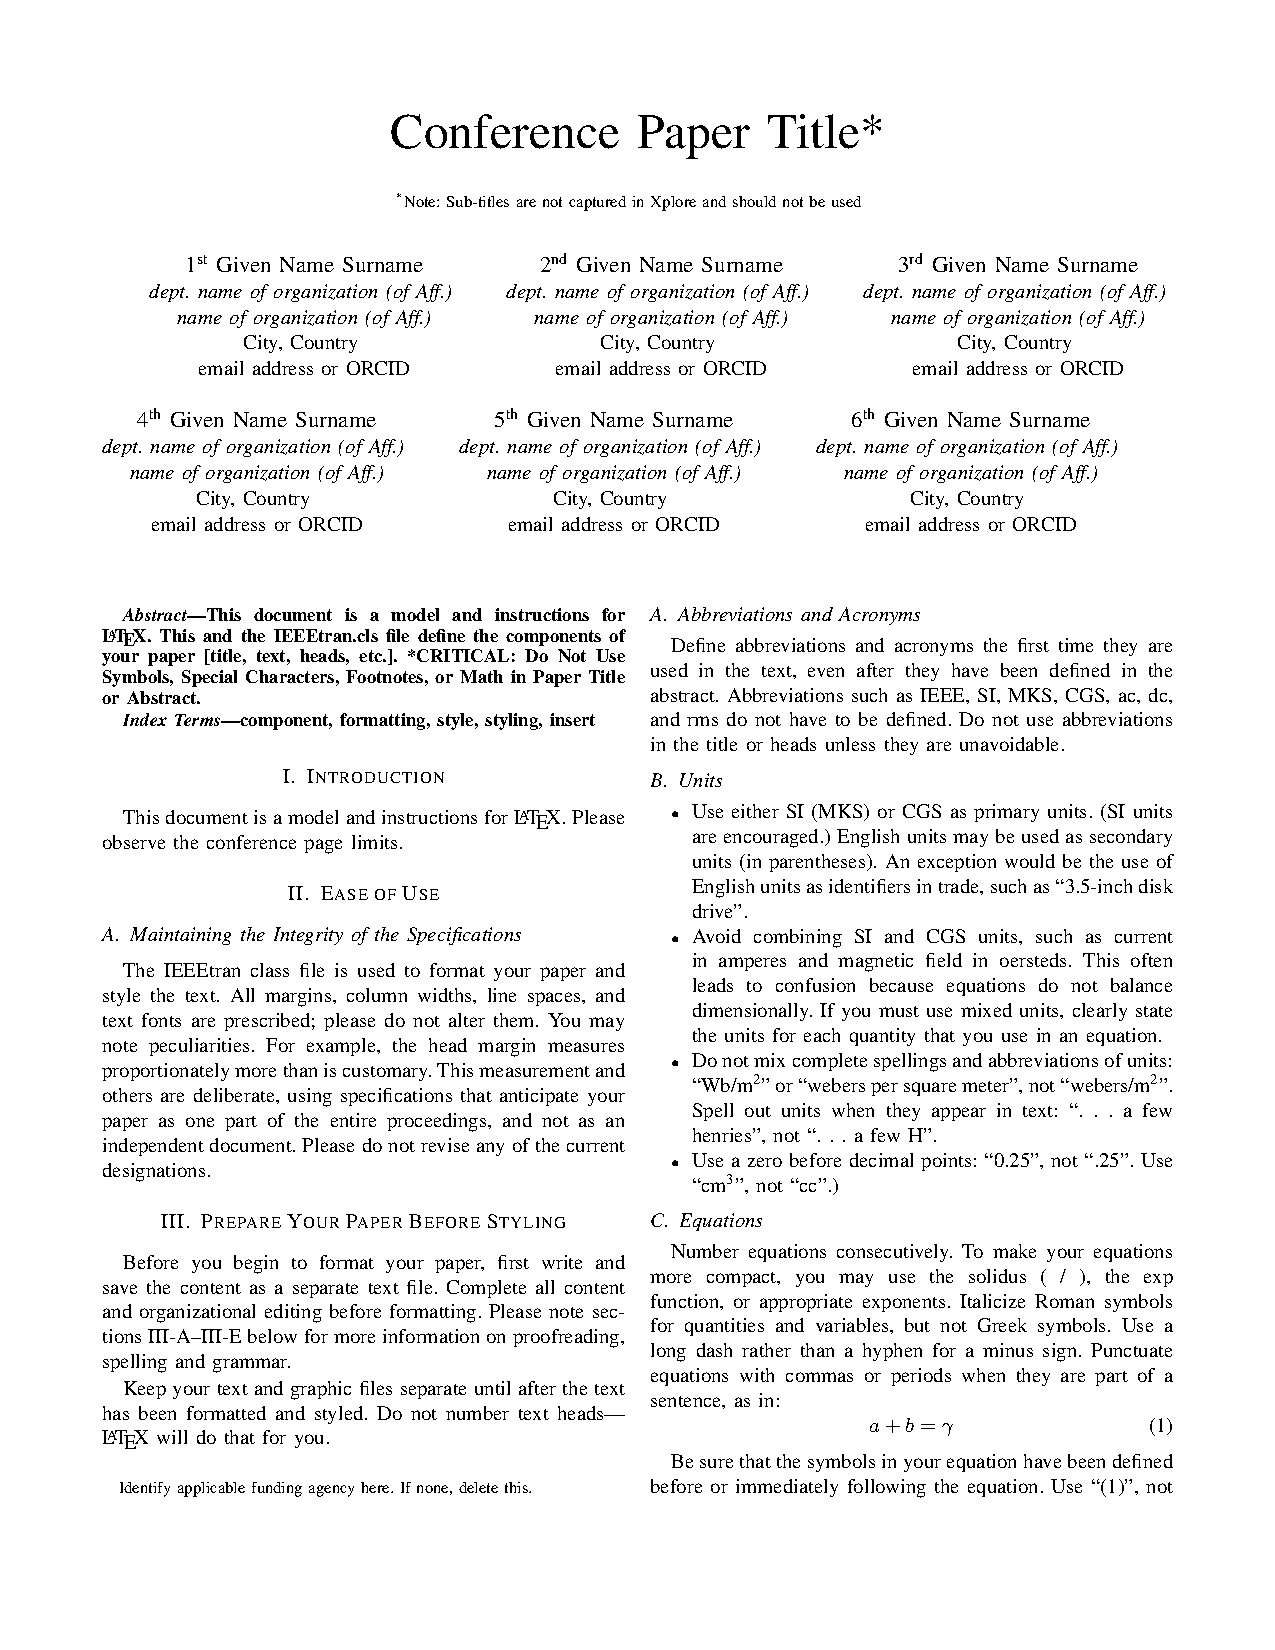
\includepdf[pages={-}]{abstract.pdf}  % Extended Abstract

\pagestyle{empty} % geen hoofding
\tableofcontents                      % Table of Contents

\newpage
\listoffigures                        % List of figures
\newpage
\listoftables % List of tables
\newpage
\listoflistings                       % List of listings (code fragments)
%
% Include the main chapters of the thesis below
%
\chapter*{Introduction}
\chaptermark{Introduction}
\addcontentsline{toc}{chapter}{Introduction}
\label{chap:intro}

One hundred years ago, Marcel Duchamp submitted his work 'Fountain' for an exhibition of the Society of Independent Artists. {add reference}
With this he forever changed how art is thought about. He forced people to re-examine the question: "What is art?", and exactly that has now become the question in AI art related work.

In so far that Kosuth has argued that art is its own definition. {Art after Philosophy}
...
The ability to be contradictory.

Style transfer you need to take into consideration that with Cubism the content is from different points-of-view.

Does it really need to go fast?
\pagestyle{fancy} %stelt de hoofding in
\graphicspath{{images/chapter1/}}

\chapter{Literature study}
\label{chap:rel_work}
In order to correctly implement a solution, we need to first understand the fundamentals.
These consist of two research fields: HPE and \gls{NST}.
The former will be used to detect poses in the art collections, but not before the latter has tried to make an improvement.
Following will be an overview of the available research in these domains.
Discussing what the goals of them are, how they achieve it, what their challenges are and their limitations.

\section{Generative Adversarial Network}
\glspl{CNN} have become the default go-to for many visual tasks and, in order to train a CNN correctly, it needs to minimize a loss function.
This is something that still requires a great amount of effort in manually crafting loss-functions.
For example, when using Euclidean distance to calculate loss during image generation, it will create a network that outputs blurry images, as minimizing Euclidean distance is achieved by averaging the output.
Having a loss-function that does what it should is a difficult problem to solve.
To sidestep these complications, Goodfellow et al. \cite{Goodfellow2014} propose a framework where the generative model competes against a discriminative model that learns to make a distinction between a sample from the real distribution and one from the generative model's distribution.
Figure \ref{fig:generative_adversarial_network} shows the architecture of a \gls{GAN}.
It consists of a generator $G$ which takes in random noise and attempts to output a sample from a specific distribution.
The discriminator $D$ will then try to distinguish between the sample from the generator and a real sample from that distribution.
A popular variation of \gls{GAN} is the \gls{cGAN}, this architecture feeds an extra label to the generator and discriminator, so that it can be conditioned to generate certain images based on the label.

\begin{figure}[h]
	\centering
	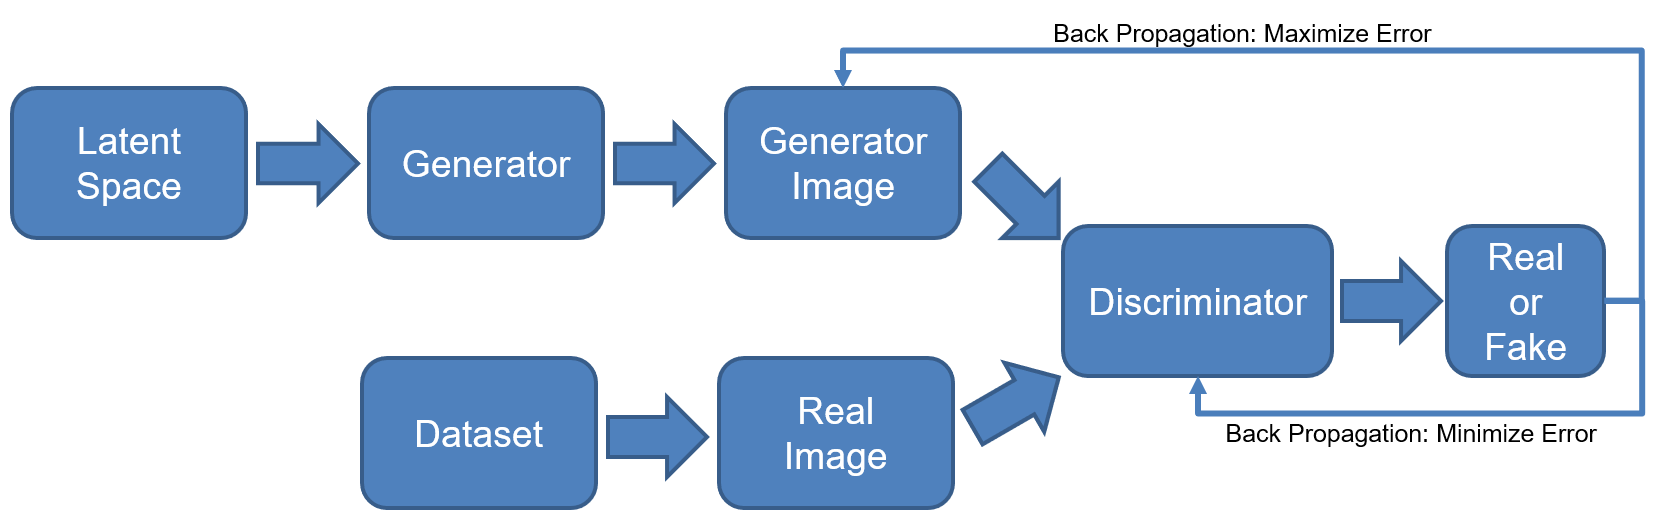
\includegraphics[width=0.8\textwidth]{generative_adversarial_network}
	\caption{The architecture of the Generative Adversarial Network \cite{GANCookbook}.}
	\label{fig:generative_adversarial_network}
\end{figure}

\section{Human Pose estimation}
\label{sec:hpe}
HPE aims to detect human features from input data such as images and videos.
It's an elementary part of computer vision with many applications among which are human action recognition (sign language), human tracking (surveillance), and human-computer interaction (video games).
This is an extensively researched area with a diverse range of different techniques.
This chapter will give an overview of all the many challenges and proposed solutions.
The focus will be on deep learning models, which have surpassed classical solutions significantly.
Specifically, around 2D HPE \cite{Munea2020, Zheng2012, Liu2104, chen2022}.

\begin{figure}[h]
	\centering
	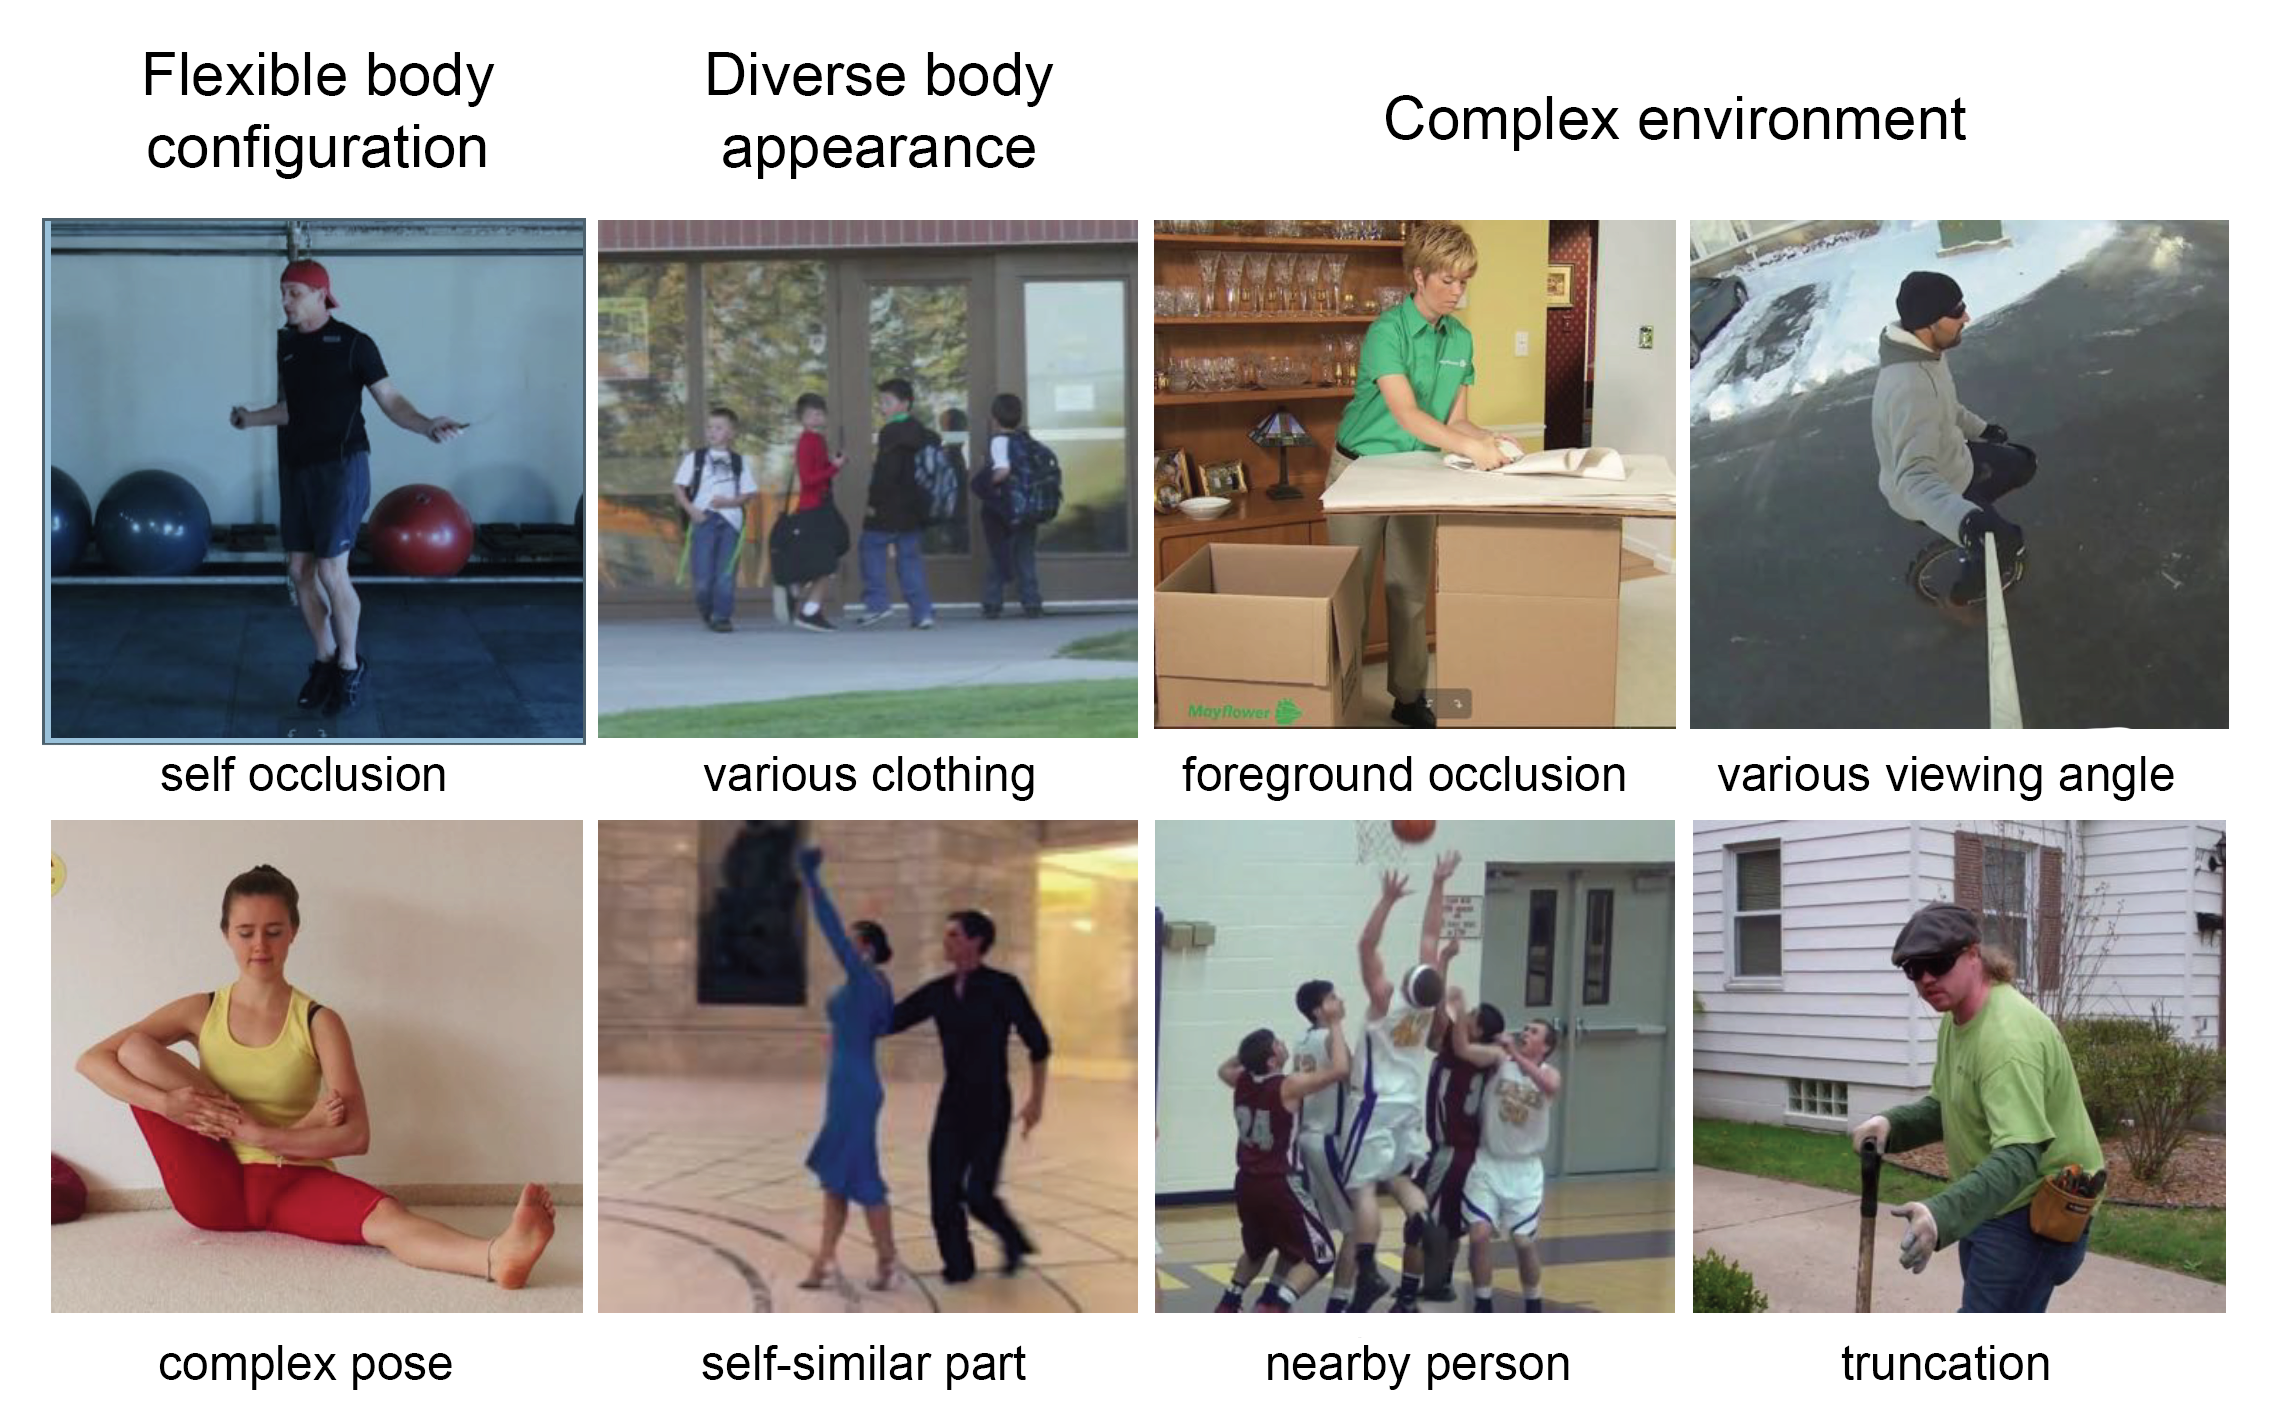
\includegraphics[width=0.6\textwidth]{hpe_problem_complexity}
	\caption{The various challenges HPE solutions face. Images from \gls{MPII} dataset. \cite{Andriluka2014, Chen2000}}
	\label{fig:hpe_problem_complexity}
\end{figure}

The human body has a high degree-of-freedom due to all the limbs, self-similar parts and body types, which may cause self-occlusion or rare/complex poses.
The variations in configuration are made even larger due to clothing, lighting, foreground occlusion, as well as viewing angles and truncation, among others.
Examples of this complexity are shown in Figure \ref{fig:hpe_problem_complexity}.
This makes HPE one of the most difficult tasks in computer vision \cite{jain2014, Chen2000}.

\begin{figure}[t]
	\centering
	\subcaptionbox{Skeleton \label{fig:pose_representation_skeleton}}{%
		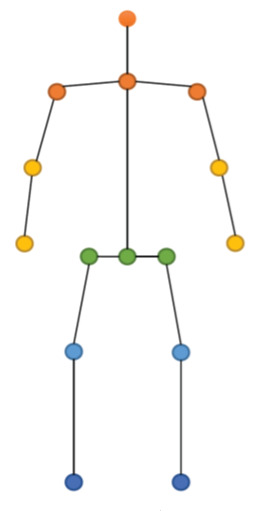
\includegraphics[width=0.15\textwidth]{pose_representation_skeleton}%
	}
	\subcaptionbox{Contour \label{fig:pose_representation_contour}}{%
		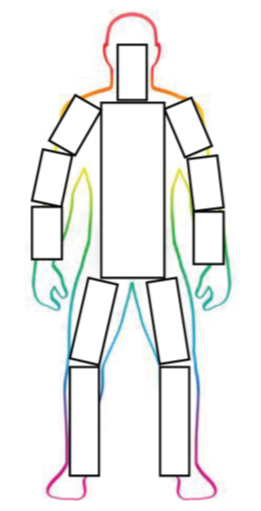
\includegraphics[width=0.15\textwidth]{pose_representation_contour}%
	}
	\subcaptionbox{Volume \label{fig:pose_representation_volume}}{%
		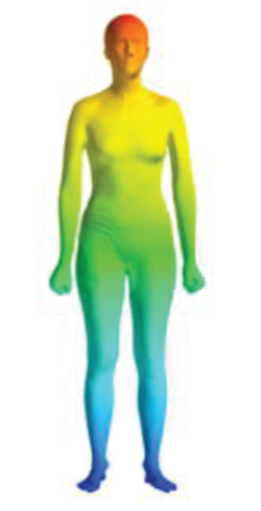
\includegraphics[width=0.15\textwidth]{pose_representation_volume}%
	}
	\caption{Models for pose representation \cite{Zheng2012}}
	\label{fig:pose_representation}
\end{figure}
\subsection{Representation}
\label{section:representation}

An important factor in HPE is how the pose will be represented.
Depending on the needs of the problem you can have a skeleton-based, contour-based, or volume-based solution \cite{Chen2000} as seen in Fig. \ref{fig:pose_representation}.

\subsubsection{Skeleton-based model}
The skeleton is made of a tree-structured set of keypoints that represent the joints of the human body.
These can be explicitly described by their coordinates in 2D or 3D space \cite{Toshev2014}.
More suitable for a CNN, however, is a heatmap which constructs a 2D Gaussian kernel around a keypoint \cite{Liu2104, SWARH}.
As they are easily implemented, they became the dominant representation.
While the skeleton-based model is a compact and flexible representation, it suffers in this aspect by not being able to hold texture or shape information \cite{Zheng2012}.

\subsubsection{Contour representation}
To capture the shape of the body parts, contour representation uses rectangles to estimate the body contours.
These methods include cardboard models \cite{Ju96}, which assumes people can be represented as a group of planar patches, and Active Shape Models \cite{COOTES95}, which tries to fit body part shapes to an image.
They were used in earlier HPE methods \cite{Chen2000}.

\subsubsection{Volume representation}
Volumetric geometric shapes can also be used as a method of representation.
Earlier methods used simple shapes like cylinders, conics, and other shapes \cite{Sidenbladh2000}.
Volume representation is a 3D mesh that represents the human body.
The most used model is Skinned Multi-Person Linear, which includes natural pose-dependent deformations imitating soft-tissue dynamics \cite{Loper2015}.  
\\
\\
For the purpose of this research, a simple model is more than adequate.
Only the most essential joints are needed to label a pose.
This makes the skeleton-based model the ideal representation to work with and will be the focus of further study.

\subsection{Datasets}
There are several publicly available datasets.
Some are outdated and will be left out, focusing only on datasets used for deep learning.

\begin{enumerate}
	\item \textbf{\gls{LSP} Dataset \cite{Johnson2010}} contains 2,000 images found on Flickr using 8 different tags looking for sport activities (athletics, badminton, baseball, gymnastics, parkour, soccer, tennis, and volleyball).
	Each person has 14 keypoints.
	An extended version was later introduced \cite{Johnson2011}, now consisting of 10,000 images. 
	For this set, they only focused on the more challenging tags (parkour, gymnastics, and athletics).
	\item \textbf{\gls{MPII} Human Pose Dataset \cite{Andriluka2014}} contains 24,290 images with 40,522 labeled people.
	They were extracted from YouTube videos found by querying for physical activities.
	Each person has 16 keypoints and it also includes occlusion labels.
	\item \textbf{\gls{COCO} Dataset \cite{Lin2014}} is a large-scale dataset for a wide range of computer vision algorithms.
	For HPE, the set contains more than 200,000 images in which 250,000 persons are annotated.
	Each person has 17 keypoints, a bounding-box and visibility labels.
	This dataset has become the most popular for benchmarking.
	\item \textbf{\gls{FLIC} Dataset \cite{Sap2013}} contains 5,003 images extracted from Hollywood movies.
	They ran a person detector which collected 20,000 images from 30 movies.
	Occluded and difficult poses were then removed leaving only 5,000 images to be annotated.
	Only the upper body received 10 keypoints.
	\item \textbf{\gls{AIC-HKD} Dataset \cite{Sap2013}} contains 300,000 images found using Internet search engines.
	In these, over 700,000 humans are annotated.
	Each person has 14 keypoints, a bounding-box, as well as visibility and left/right labels.
	\item \textbf{CrowdPose Dataset \cite{Li2018}} puts an emphasis on crowded images.
	30,000 images from \gls{MPII}, gls{COCO} and gls{AIC-HKD} were measured with a Crowd Index, which evaluates the crowdedness.
	Finally, 20,000 images are selected and 80,000 persons annotated.
	Each person has 14 keypoints and a full-body bounding box.
	\item \textbf{Human-Art Dataset \cite{Ju2023}} bridges the gap between natural and artificial images.
	The set contains 50,000 high-quality images with 123,000 annotated humans.
	Each person has 17 keypoints, bounding boxes, self-contact points, and text information.
\end{enumerate}

\subsection{Discriminative Methods and Generative Methods}
Before deep learning became prominent in HPE, there were already a number of different methods in use.
Some of these methods are compatible with the deep learning methods and were promptly adopted.
An early distinction is between generative and discriminative methods.

\textbf{Generative Models} work with prior beliefs about the pose.
More information about this can be found in the section about representation \ref{section:representation}.
It will project the pose on the image and verify it with the image data.
If it doesn't comply, the pose is adjusted using descent directions found by minimizing an error function to converge to a local optimization \cite{Pons-Moll2011}.

\textbf{Discriminative Models} on the other hand, try to map the pose on the image data with learned models.
There are several methods in this category, among which are the deep learning-based methods.
The deep-learning methods are further categorized by the following sections.

\subsection{Single-Person Pose Estimation Methods}
Single-person pose estimation tries to evaluate only one pose from an image.
There are two major methods that are in use: regression methods and detection-based methods.

\textbf{Regression-based Methods} learn a network that maps all the body keypoints to the image directly, as shown in Figure \ref{fig:single_pose_estimation_regression_methods}.
The first successful deep learning model came from Toshev and Szegedy \cite{Toshev2014} and is considered the switch in paradigm from classic approaches to deep learning HPE.
Based on AlexNet for its simple but effective architecture \cite{AlexNet}, they use a seven-layered model with five convolution layers and two fully-connected layers for the pose regressor.
They then cascade the resulting found keypoints to the next stage where it refines it using the area around the keypoints.
While the network is the same, the different stages will have different learned parameters.
With every stage, the found keypoints become more accurate.
Carreira et al. \cite{CarreiraAFM15} introduce an Iterative Error Feedback which is a self-correcting model using top-down feedback.
Using the image and a starting pose modeled as a heatmap, the model, based on GoogLeNet \cite{googlenet}, will predict an error for each keypoint.
The pose is then corrected based on the error and fed into the next module as a heatmap with the input image.
With each iteration it converges towards the solution instead of making the prediction in one go.
Regression-based methods map the keypoints directly on the image, making it a non-linear problem, which leads to a less robust generalization \cite{Liu2104}.

\begin{figure}[h]
	\centering
	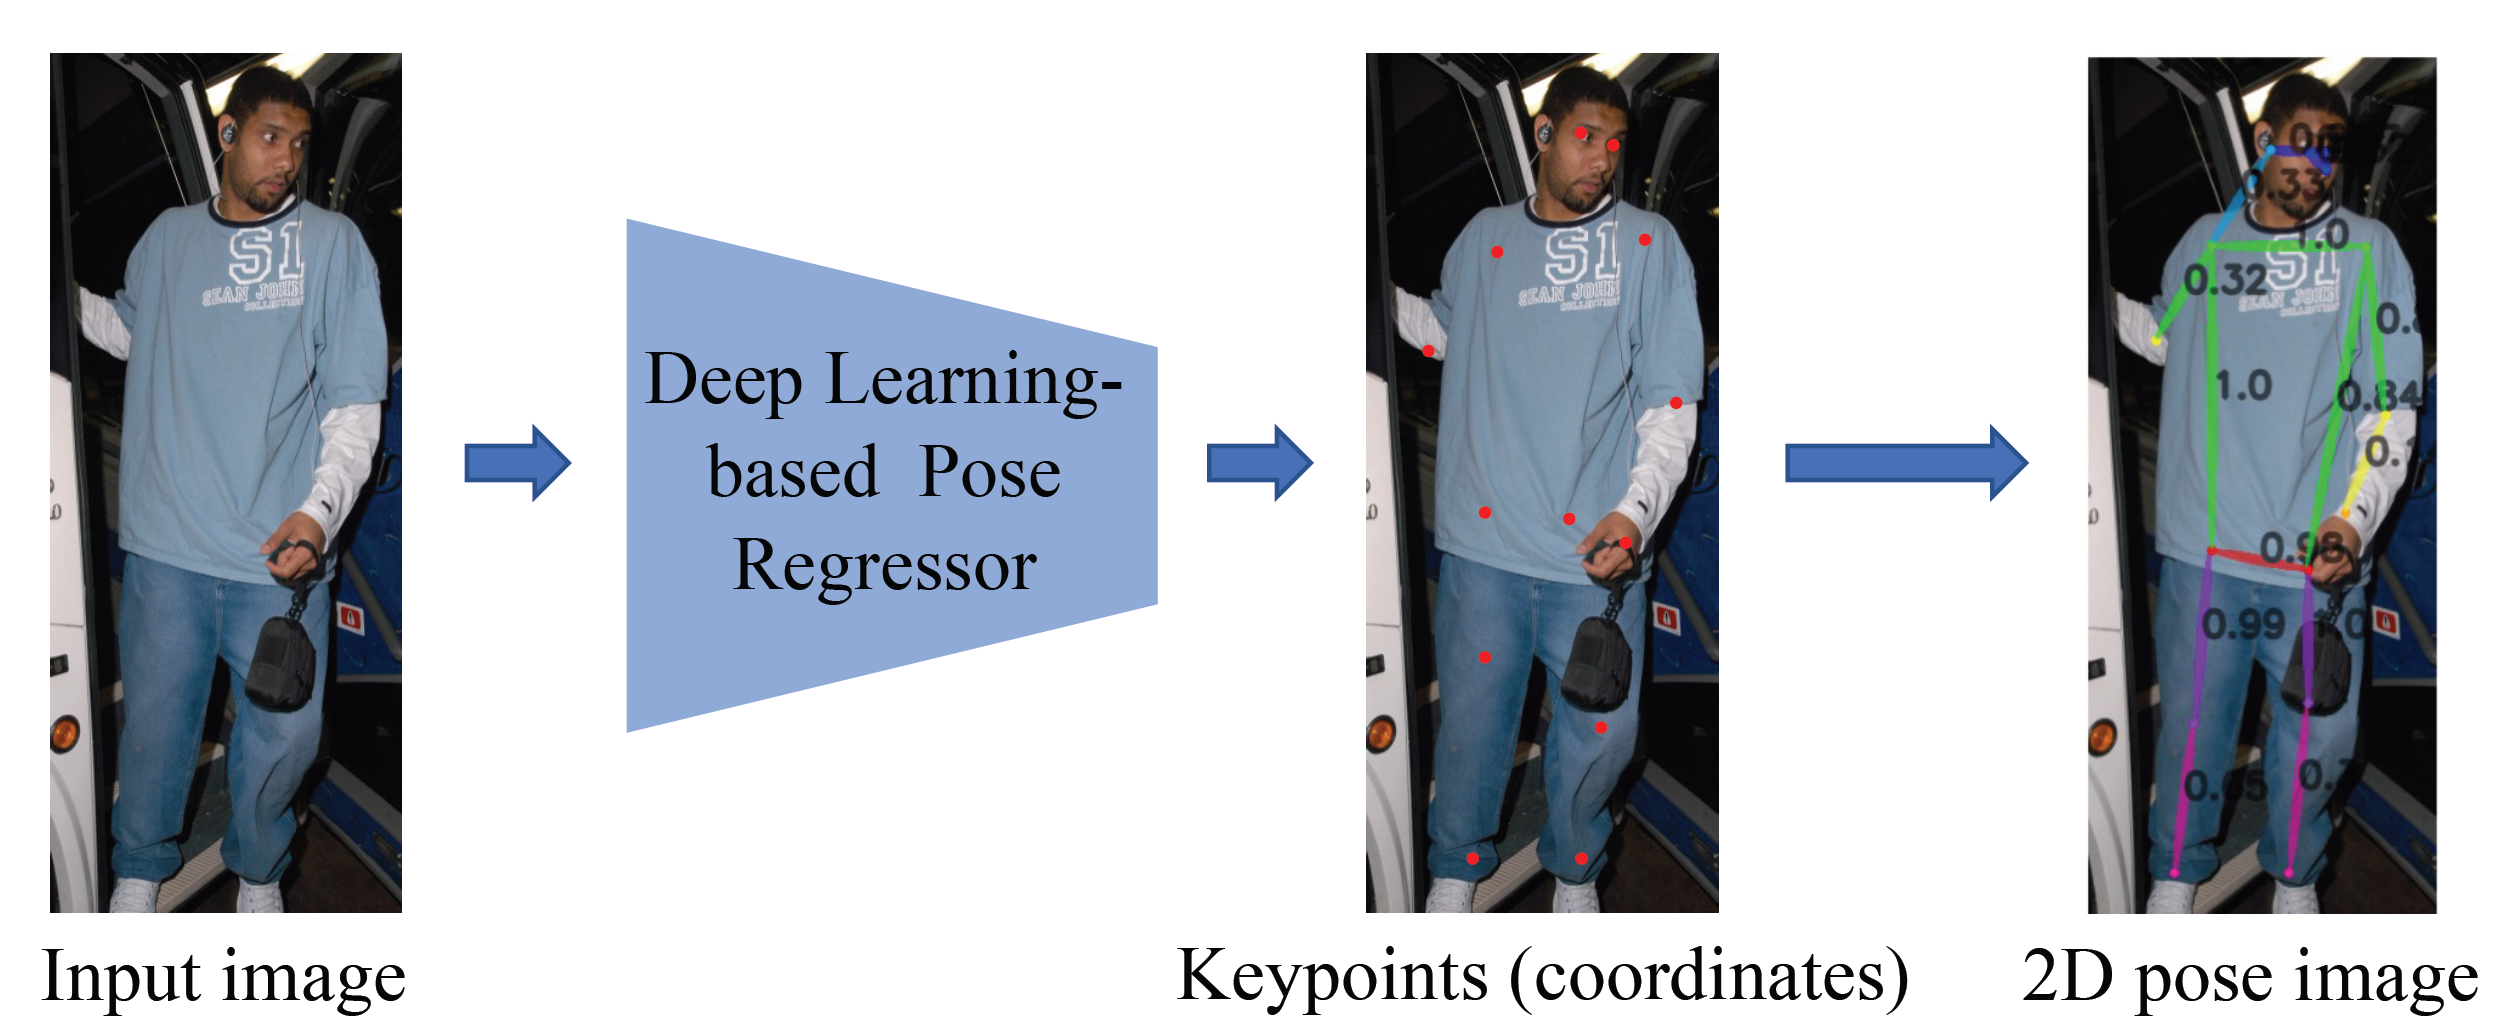
\includegraphics[width=0.6\textwidth]{single_pose_estimation_regression_methods}%
	\caption{Single-Person HPE Regression Methods as presented in \cite{Zheng2012}}
	\label{fig:single_pose_estimation_regression_methods}
\end{figure}

\textbf{Heatmap and Detection-based Methods} will first estimate the individual body parts using heatmaps.
This method results in an easier optimization and a more robust generalization \cite{chen2022}.
Most of the latest HPE methods use heatmaps because of this.
After the joints are found, they are assembled to fit a human skeleton, as shown in Figure \ref{fig:single_pose_estimation_heatmap-based_methods}.
Tompson et al. \cite{TompsonJLB14} proposed a hybrid architecture where the detection of body parts is handled by a CNN and a Spatial-Model to bring those together.
The first step produces many false-positives which are removed in the second step by restricting joint inter-connectivity to enforce correct anatomy.
They build on this in \cite{Tompson2015} where they use a cascade to refine predictions.

\begin{figure}[h]
	\centering
	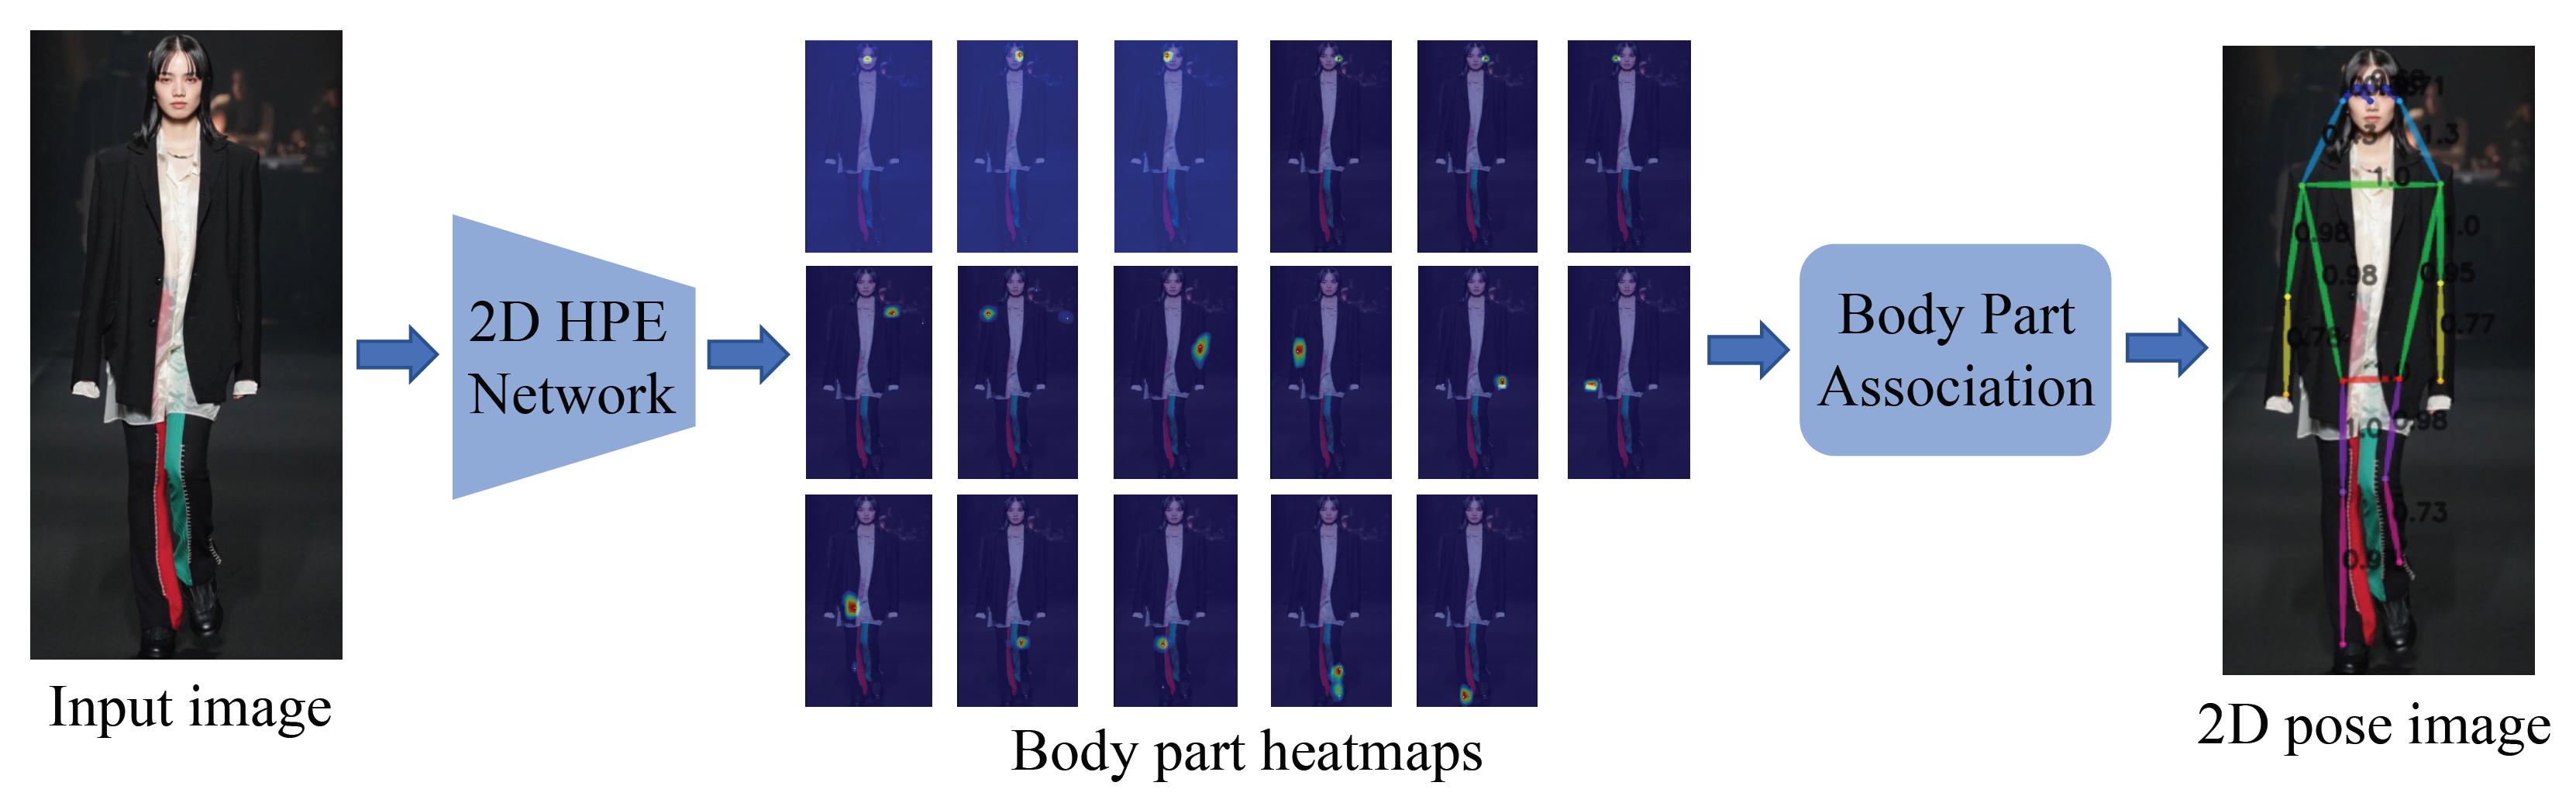
\includegraphics[width=0.8\textwidth]{single_pose_estimation_heatmap-based_methods}%
	\caption{Single-Person HPE Heatmap-based Methods as presented in \cite{Zheng2012}}
	\label{fig:single_pose_estimation_heatmap-based_methods}
\end{figure}

A fundamental work written by Wei et al. \cite{Wei2016} combines convolution networks with Pose Machines \cite{Ramakrishna2014}.
Pose Machines is an iterative architecture which consists of two models:
The first is used for stage one where it predicts potential heatmaps for the joints.
The second model is used for subsequent stages where the result of the previous stage is fed in together with the results of its own convolution network on the input image. 
This gradually refines the predictions for the joints and their positioning.
Another influential work was being written at the same time by Newell et al. \cite{Newell2016}.
Similar to \gls{CPMs}, this is also an iterative architecture.
They suggest what they call a "stacked hourglass" network, where "hourglass" modules are repeated.
In an "hourglass" module, first, the features are downsampled and, afterwards, upsampled again.
This network captures different spatial relationships between joints at different resolutions.
Several other works \cite{Yang2017, Chou17} have since improved on the network design.
Both use intermediate supervision to tackle the problem of vanishing gradients.
This still doesn't build a deep sub-network for feature extraction which limits the predictions.
This has become less of a problem with the emergence of the \gls{ResNet} \cite{He2015} which allows better back-propagation at deeper levels through shortcuts.

\begin{figure}[h]
	\centering
	\subcaptionbox{HRNet \label{fig:single_pose_estimation_HRNet}}[0.39\textwidth]{%
		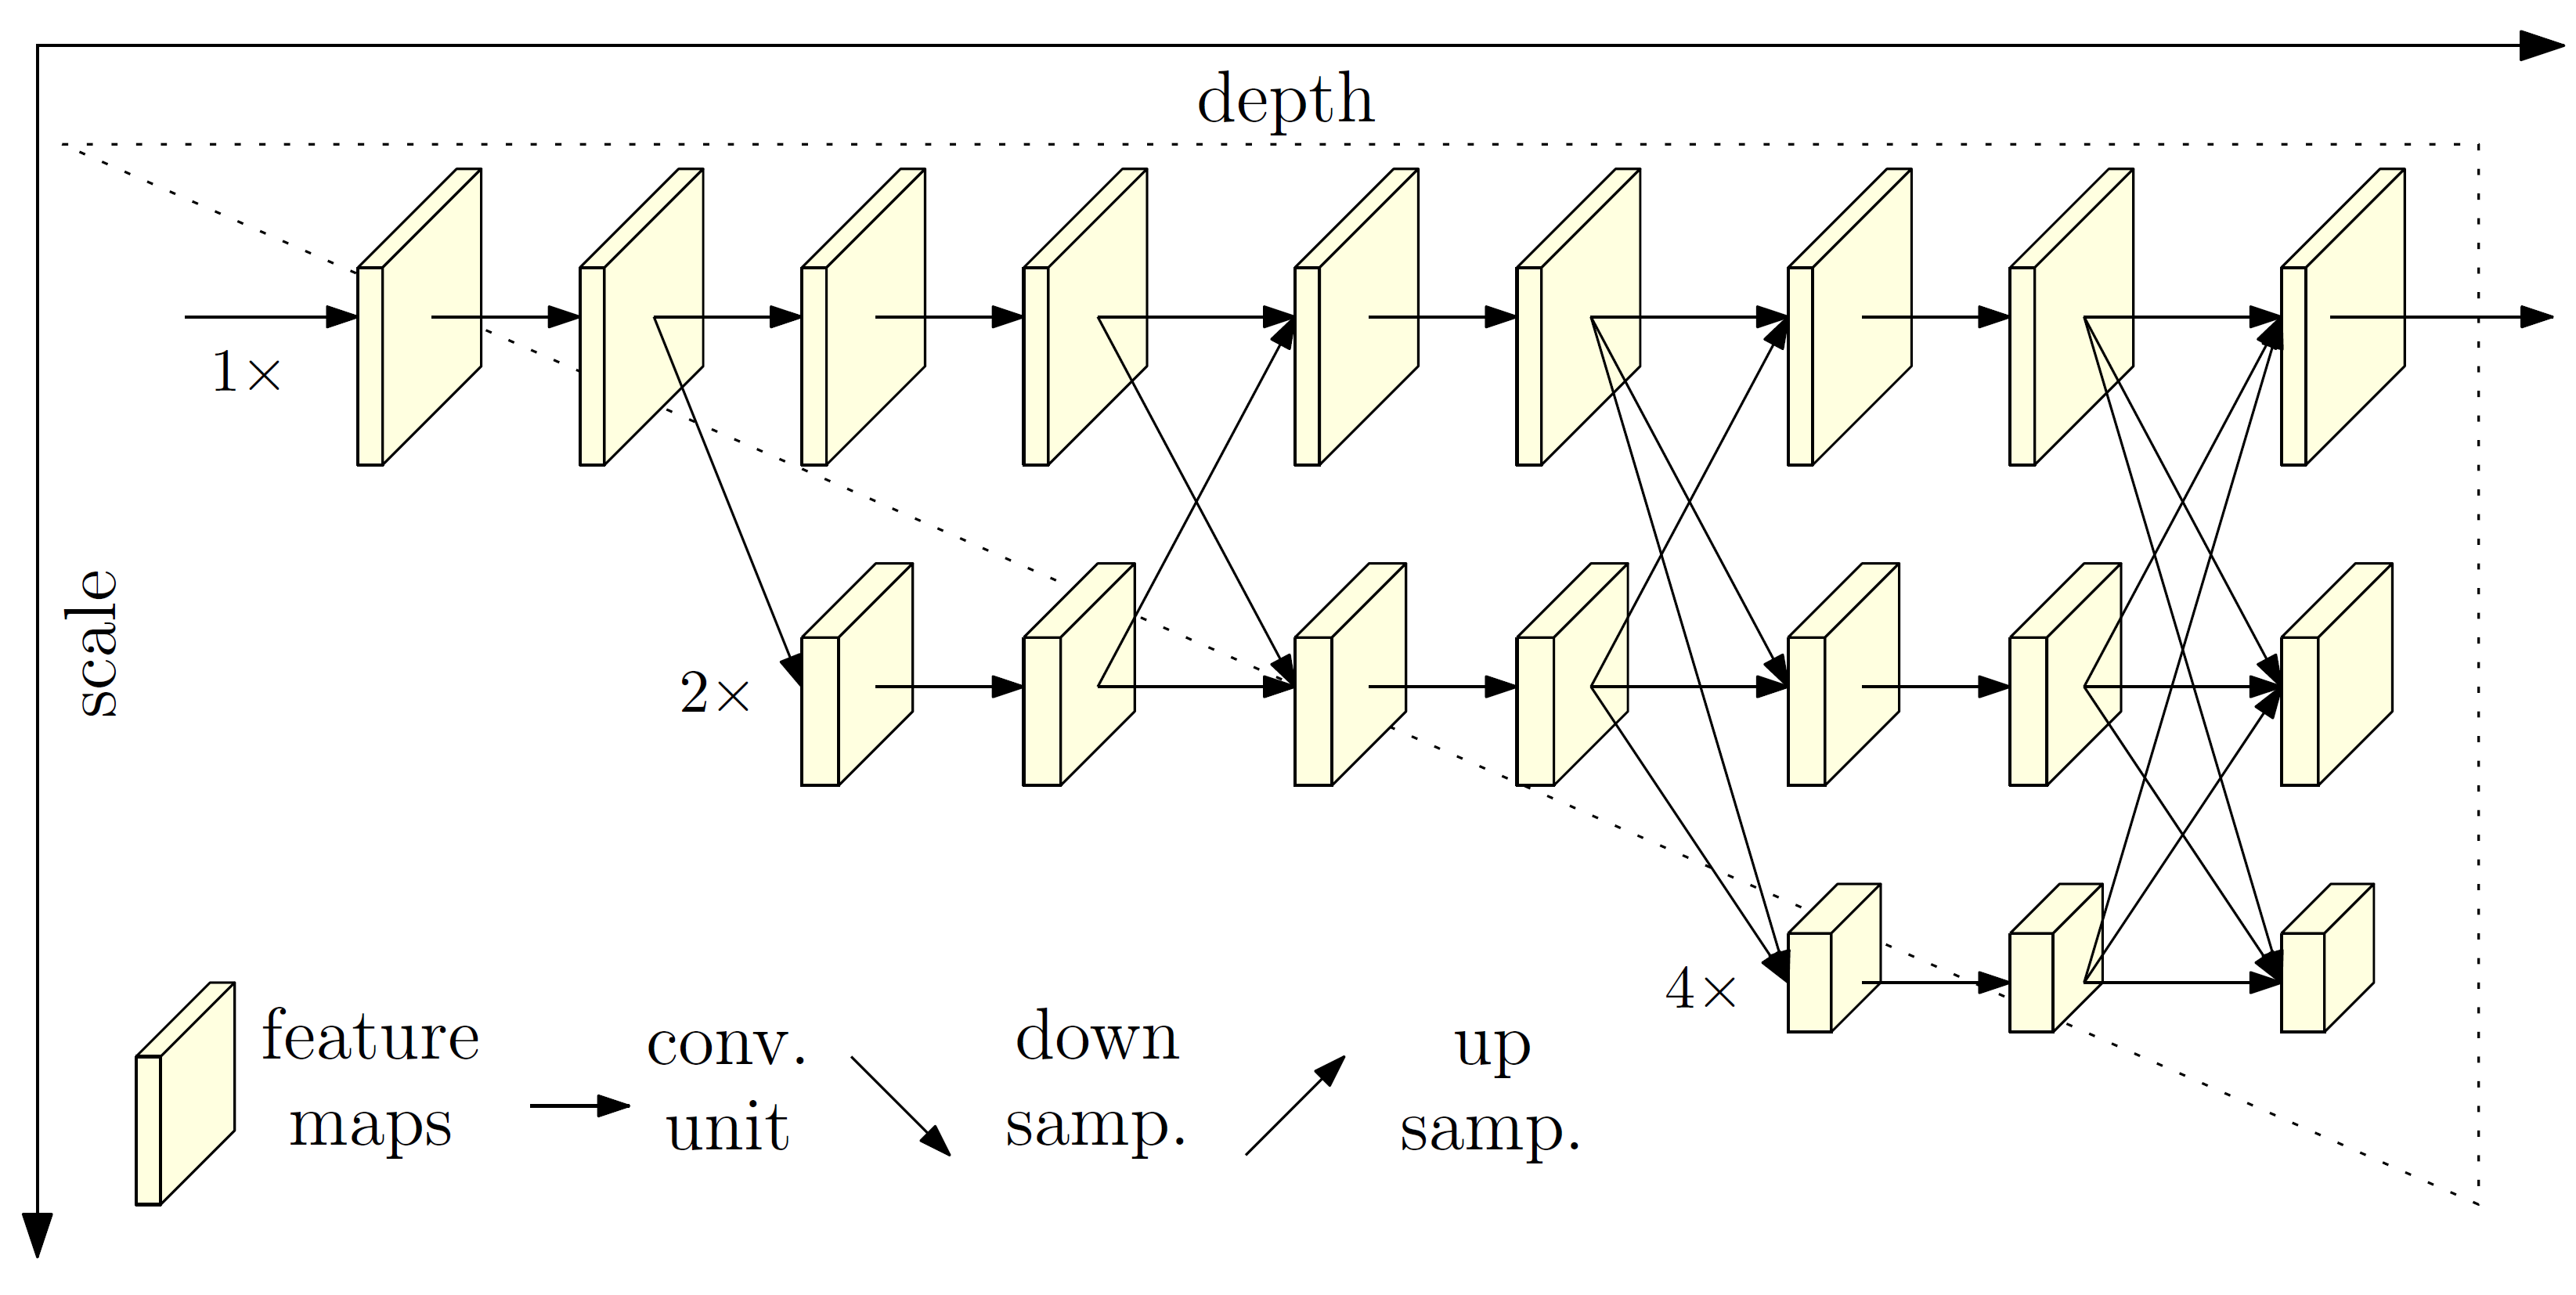
\includegraphics[width=0.39\textwidth]{single_pose_estimation_HRNet}%
	}
	\subcaptionbox{Multi-Scale Fusion \label{fig:single_pose_estimation_multi-scale_fusion}}[0.59\textwidth]{%
		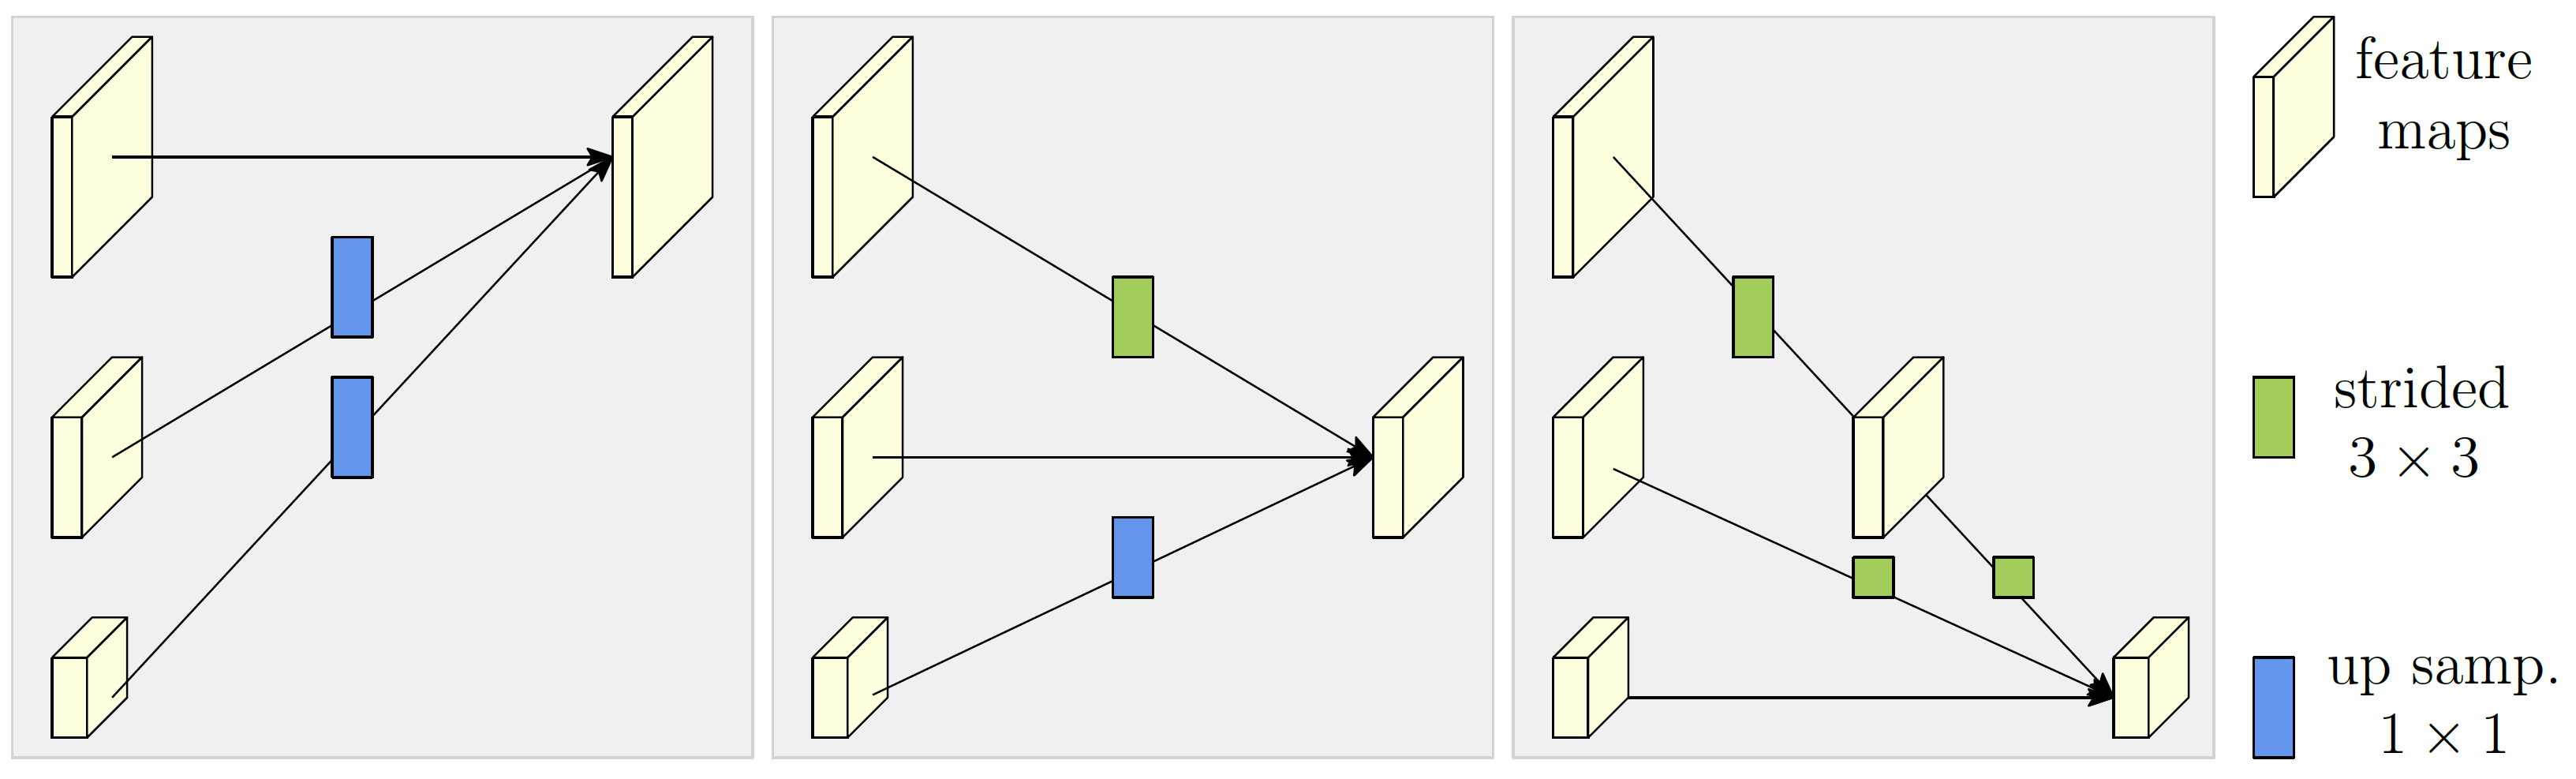
\includegraphics[width=0.59\textwidth]{single_pose_estimation_multi-scale_fusion}%
	}
	\caption{
		The architecture of the High-Resolution network and how it applies multi-scale fusion \cite{Sun2019}.
	}
	\label{fig:HRNet}
\end{figure}

A more recent work by Sun et al. \cite{Sun2019} maintains high-resolution representations instead of working with the high-resolution from the low-to-high sub-network.
After a first high-resolution sub-network, it gradually adds high-to-low sub-networks in parallel to predict multi-resolution features.
Before each branch, they apply multi-scale fusion, which joins the predicted features from each scale on each other scale (Figure \ref{fig:HRNet}).
This network has proven very effective and inspired several variations \cite{Cheng2019, Yu2021, Yuan2021}.
Chen et al. \cite{Chen2017b} propose using \gls{cGAN} \cite{Mirza2014} to improve constraints of joint inter-connectivity and infer occluded body parts.
A structure-aware convolution network using a stacked hourglass serves as generator which generates pose heatmaps as well as occlusion heatmaps for each joint.
Two discriminators are used, one to discriminate between low- and high-confidence predictions, another for real and fake poses.
A more classic GAN is used by Chou et al. \cite{Chou2017}, where they use a stacked hourglass network for both the generator as the discriminator.
The generator predicts the heatmaps for each joint and the discriminator distinguished between the real and fake ones.

\subsection{Multi-Person Methods}
With multi-person methods comes an extra layer of difficulty; they need to detect each person separately.
To solve this problem multi-person methods propose several solutions. 
The two most popular are top-down and bottom-up methods.

\textbf{Top-Down Methods} will first try to detect all persons in the image with a human detector.
Each person is cropped by the bounding box and a single-person estimator predicts a pose.
Occlusion and truncation are a regular occurrence in multi-person scenes and an inevitable problem.
One of the early multi-person models, by Iqbal et al. \cite{Iqbal2016}, creates a robust model against occlusion.
It uses \gls{Faster R-CNN} \cite{Ren2015} to detect the human boundaries, after which it applies integer linear programming on each person's fully connected graph to obtain the final pose estimates.
This technique is similar to \cite{Pishchulin2015}, but, instead of working on all globally found joints, it only considers local joints.
It can also handle any kind of occlusion or truncation.
The use of a human detector comes with its own set of problems, which Fang et al. \cite{Fang2016} try to remedy with \gls{RPME}.
Their solution consists of two components:
They try to tackle inaccurate bounding boxes with a Symmetric Spatial Transformer Network and redundant detections with Parametric Pose Non-Maximum-Suppresion.
They also propose a 3rd component, the Pose-Guided Proposals Generator, which can augment training samples.
Papandreou et al. \cite{Papandreou2017} use a two stage pipeline.
In the first stage, they employ the Faster R-CNN detector.
In the second stage, they estimate the pose in each found bounding box using their own network.
It predicts heatmaps using a fully convolutional \gls{ResNet} and then uses their own novel aggregation procedure.
Afterwards, they do post-processing using keypoint-based \gls{NMS}; a method of their own making.
A continuous effort is taken by Chen et al. \cite{Chen2017a} to deal with occlusion and truncation.
They suggest a two stage architecture, where first the "simple" keypoints are captured with GlobalNet, a feature pyramid network based on \cite{Lin2016}, and the "hard" keypoints are handled by their RefineNet.
It integrates the information via upsampling and concatenating of HyperNet \cite{Kong2016} and using an adapted stacked hourglass.
They achieved great results and several others improved on their work \cite{Su2019, Li2019a}.
In more recent research, a new method was become competitive with \glspl{CNN}.
Based on work in language modeling, attention mechanisms, an optimization of recurrent networks, allow the modeling of dependencies without regard of the distance in the input or output sequences.
The Transformer, introduced by Vaswani et al. \cite{Vaswani2017}, eliminates recurrence and relies solely on attention mechanisms.
This enables it to work better in parallel while it still maintains state-of-the-art performance.
Based on this new architecture, Dosovitskiy et al. \cite{Dosovitskiy2020} created a new model that can work with images; the \gls{ViT}.
Xu et al. \cite{xu2022} use the vision transformer to apply it to the HPE task.
As seen in Figure \ref{fig:vitpose}, they try to keep the network simple and don't use certain optimizations that can increase complexity.
It works by splitting the input image into fixed-size patches which are linearly embedded and then fed into the transformer blocks.
The output of this is then processed by different decoders to form the heatmaps.
To show the strong representation ability of transformers the authors provide a simple decoder next to the classic decoder and show that even the simple decoder obtains competitive results.

\begin{figure}[h]
	\centering
	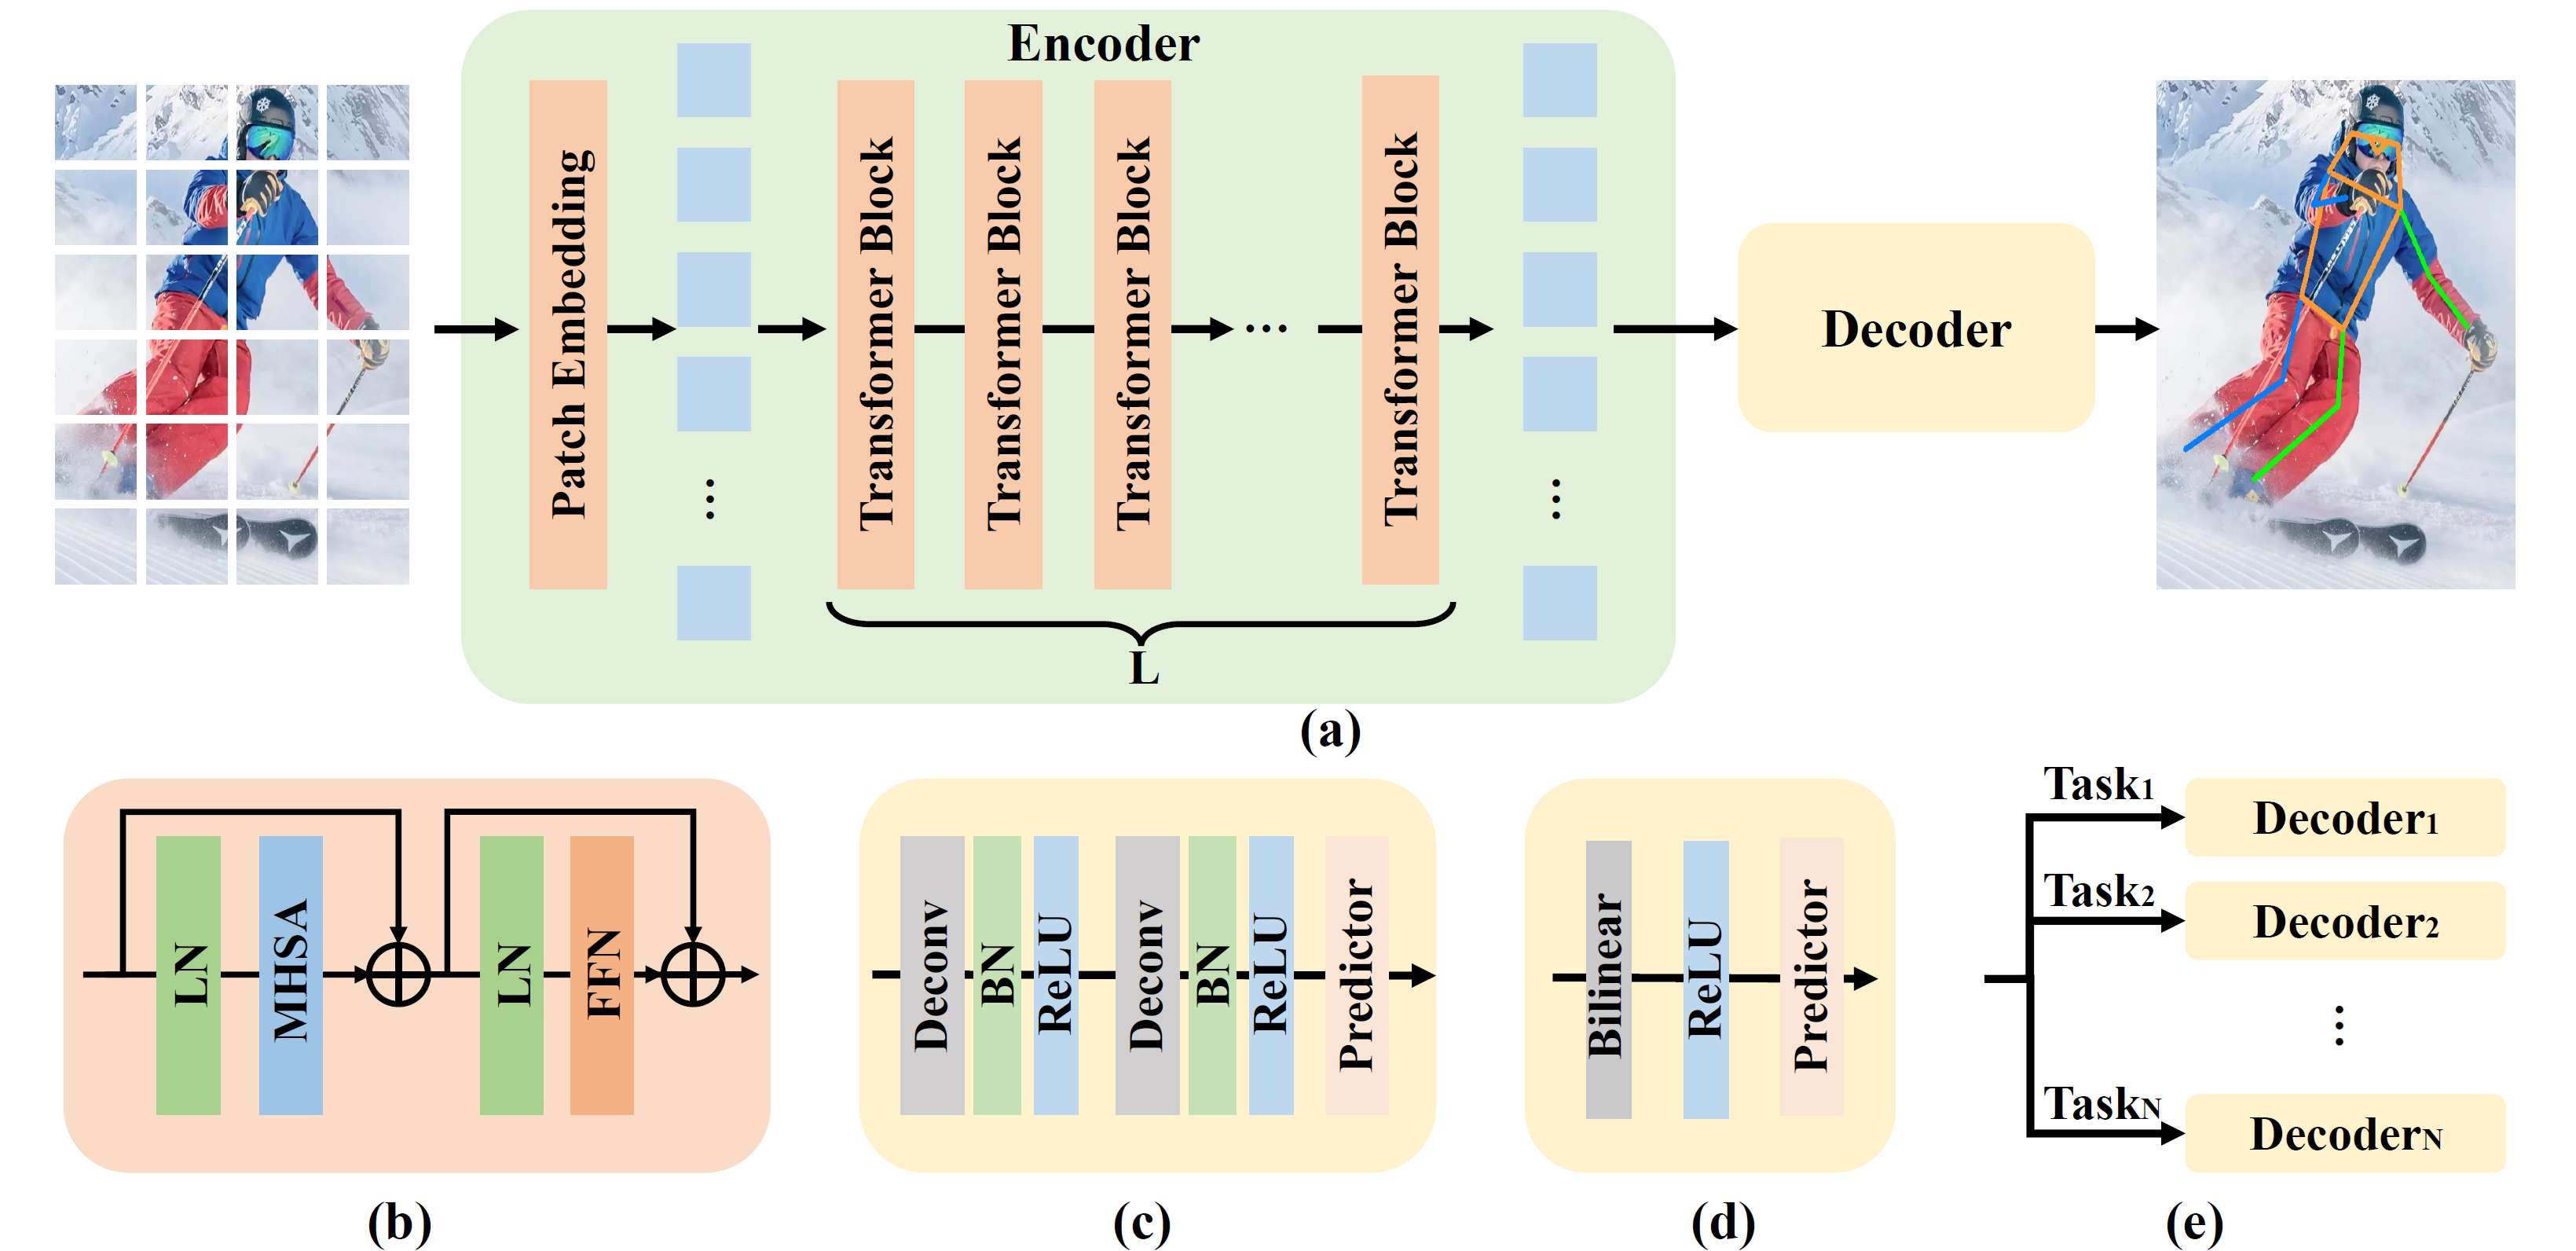
\includegraphics[width=0.8\textwidth]{vitpose}%
	\caption{
		(a) The framework of ViTPose. (b) The transformer block. (c) The classic decoder. (d) The simple decoder. (e) The decoders for multiple datasets. \cite{xu2022}
	}
	\label{fig:vitpose}
\end{figure}

\textbf{Bottom-Up Methods} use a different approach to predict the keypoints.
They first locate all joints in the image and then afterwards assemble them in potential poses.
DeepCut by Pishchulin et al. \cite{Pishchulin2015} is one of the first multi-person models using \glspl{CNN}.
Using Fast R-CNN \cite{Ren2015}, it detects the body parts and labels each.
With the joints found, it then uses \gls{ILP} to assemble them.
However, this method is very computationally expensive; NP-hard.
Insafutdinov et al. \cite{Insafutdinov2016} therefor introduce a stronger part detector and better optimization strategy with DeeperCut.
\gls{CPMs} make a return with OpenPose by Cao et al. \cite{Cao2018}.
They're used to predict the joints with heatmaps and \glspl{PAFs}.
PAFs also encodes the position and orientation of the limb which makes the assembly of joints into different poses more reliable.
They can achieve real-time results with this method, and several others have improved on their design \cite{Zhu2017a, Hidalgo2019, Li2019b}.
The high performance is only applicable to high-resolution images and low-resolution images or images with occlusions perform poorly.
Kreiss et al. \cite{Kreiss2019} continue on the idea of fields and introduce the \gls{PIF} and \gls{PAF}.
First, they predict the location of the different joints with \gls{PIF}.
Afterwards, they use \gls{PAF} to find the inter-joint relationships.
They are able to outperform any previous OpenPose-based proposals on low-resolution and occlusions.
Newell et al. \cite{Newell2016-2} introduce associative embedding which is a new method to represent the output.
This is a single-stage architecture as opposed to the two-staged architectures previously discussed.
They make use of the stacked hourglass network from \cite{Newell2016} with some small modifications, and produce joint heatmaps and associative embedding tags.
Continuing on the idea of associative embedding, Cheng et al. \cite{Cheng2019} use HRNet \cite{Sun2019} as backbone for their HigherHRNet (Figure \ref{fig:higherhrnet}).
Their method focuses on the scale-variance problem; a problem which hasn't been studied much, so it can localize keypoints for small persons better.
Lou et al. \cite{Lou2020} introduce \gls{SAHR} and \gls{WAHR} to the scale-variance problem.
\gls{SAHR} adaptively adjusts the standard deviation of each heatmap corresponding with the scale of the person.
\gls{WAHR} rebalances the foreground and background samples, so \gls{SAHR} can work to its fullest extent.

\begin{figure}[h]
	\centering
	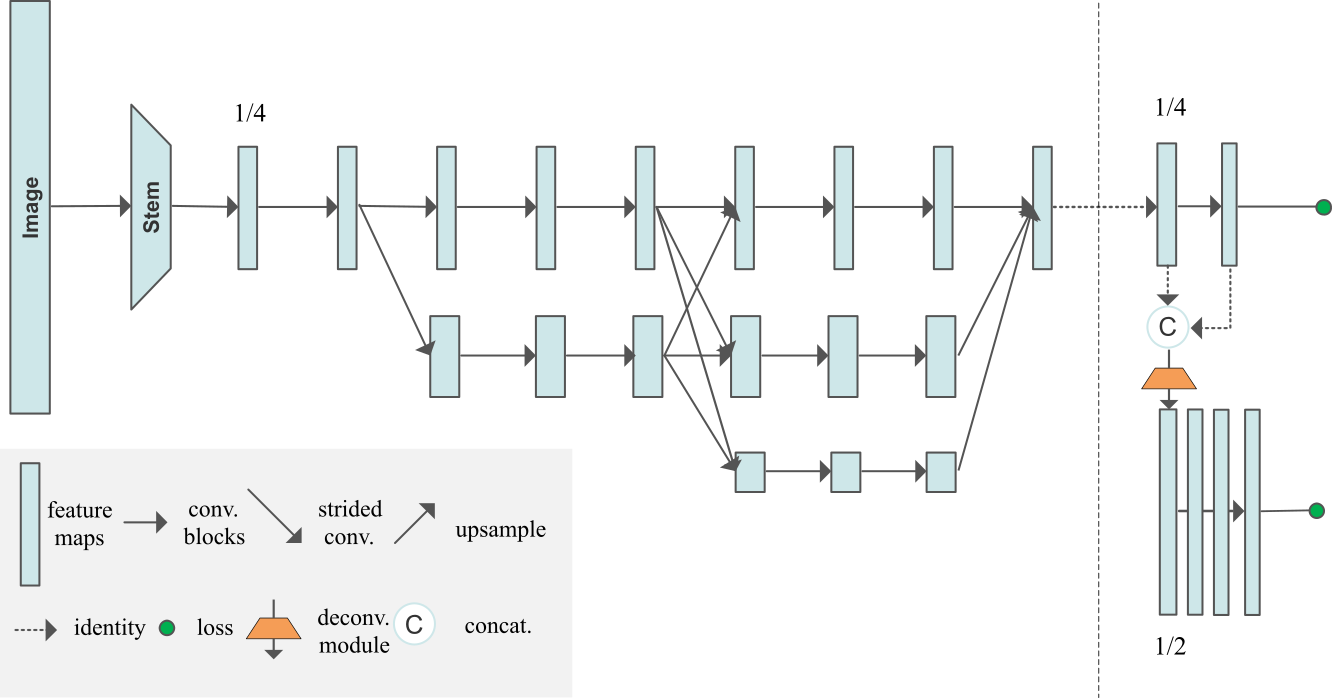
\includegraphics[width=0.5\textwidth]{higherhrnet}%
	\caption{
		The architecture of HigherHRNet. It uses HRNet as backbone. \cite{Cheng2019}
	}
	\label{fig:higherhrnet}
\end{figure}

\subsubsection{Summary}
An important challenge for HPE is making predictions in scenes with hight occlusions.
Top-down models achieve state-of-the art performance on almost all benchmark datasets \cite{Chen2000}.
However, they have difficulty with overlapping bodies and human detectors add an extra layer of failure.
To the same extent, bottom-up models have greater inaccuracy when grouping in occluded scenes.
Computationally, the top-down model's speed is heavily bound to the number of people the human detector finds.
The higher efficiency of bottom-up models make them more suitable for real-time applications.

\subsection{Evaluation Metric}
The evaluation of an HPE looks to measure the accuracy of the location of predicted joints.
Because of the different number of features and tasks across datasets, there are also several different evaluation metrics in use.
Explained next will be the most commonly used metrics.

\begin{enumerate}
	\item \textbf{Percentage of Correct Parts (PCP)}, proposed by Ferrari at al. \cite{Ferrari2008}, measures the detection rate of limbs.
	A limb is considered the area between two joints and viewed as detected when the distance between the predicted joints and the real joints is less than halve the length of the limb.
	This method penalizes shorter limbs and to address this, \gls{PDJ} was introduced which instead measures it with a fraction of the torso diameter.
	The higher, the better.
	\item \textbf{Percentage of Correct Keypoints (PCK)}, suggested by Yang et al. \cite{Yang2013}, measures the accuracy of the predicted keypoints.
	The keypoints should be within a certain threshold, which is a fraction of the person's bounding box size; denoted as PCK@0.2 when it should be less than 20\%.
	It can also be 50\% of the head's length; denoted as PCKh@0.5, which makes it "articulation independent".
	The higher, the better.
	\item \textbf{Average Precision/Recall (AP/AR)}, by Yang et al. \cite{Yang2013}, is calculated by counting a keypoint that is within a certain threshold of the ground truth as a true positive.
	For Lin et al. \cite{Lin2014}, the AP is calculated by measuring the \gls{OKS} (Figure \ref{fig:keypoint-similarity-distribution}) which is similar to Intersection over Union in Object Detection.
	The \gls{OKS} is defined as:
	\begin{equation}
		\operatorname{OKS} = \frac{\sum_{i}\exp(-d_i^2/2s^2k_i^2)\delta(v_i > 0)}{\sum_i \delta(v_i > 0)}
	\end{equation}
	Here, $d_i$ is the distance between the predicted keypoint and the ground truth.
	The distance is run through a unnormalized Gaussian with a standard deviation of $sk_i$ which yields a similarity that ranges between 0 and 1.
	$s$ is the scale, calculated as the root of the segment area, and $k_i$ is a constant for each keypoint that controls falloff.
	\gls{OKS} is the mean of visible keypoints ($v_i > 0$).
	These can be used to calculate \gls{AP} and \gls{AR} at different thresholds.
	10 different metrics are used to calculate the performance of a model:
	$\operatorname{AP}^{0.5}$ (where the $\operatorname{OKS}$ threshold is $0.5$), $\operatorname{AP}^{0.75}$ and $\operatorname{AP}$ (the mean of 10 values from $\operatorname{OKS}=0.50$ to $0.95$ with a $0.05$ step), as well as, $\operatorname{AP}^{M}$ for medium scaled objects and $\operatorname{AP}^{L}$ for large scaled objects.
	The same metrics are calculated for \gls{AR}.
	The higher, the better.
\end{enumerate}

\begin{figure}[h]
	\centering
	\captionbox{
		\label{fig:keypoint-similarity-distribution}
		An illustration of keypoint similarity.
		The predicted values (red and green) are at the same distance from the ground-truth (blue).
		The wrist and eye have a different $k_i$ causing a different falloff \cite{Ronchi2017}.
	}[0.86\textwidth]{
		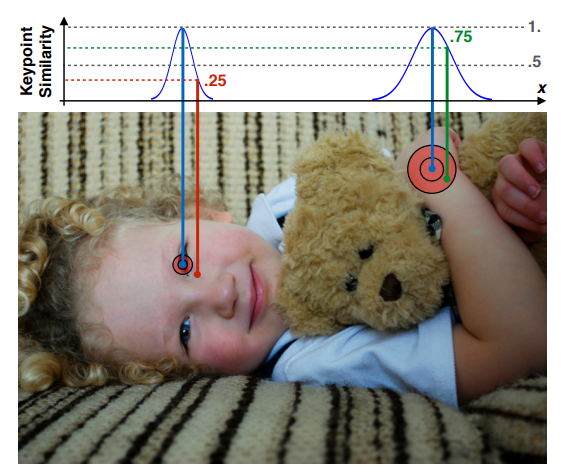
\includegraphics[width=0.5\textwidth]{keypoint-similarity-distribution}%
	}
\end{figure}

\section{Image Style Transfer}
Image Style Transfer is the technique of applying the style of one image to the content of another.
Traditionally, this is a problem reserved for only artists, but more recently this has also interested computer scientists.
There are several different ideas on how this can be achieved,
ranging from how to separate the style from the content to how well an algorithm can generalize.
An overview of all the different challenges and solutions will be given in this chapter.

\subsection{Datasets}
Due to a lack of benchmark datasets, multiple papers will mix and match from different datasets, like \gls{COCO} or ImageNet \cite{Deng2009}.

\begin{enumerate}
	\item \textbf{Cityscape Dataset \cite{Cordts2016}} consists of 2975 images of cityscapes with semantic annotations.
	\item \textbf{Facades Dataset \cite{Tylecek2013}} consists of 400 images of building facades with architectural annotations.
	\item \textbf{Maps Dataset \cite{Isola2016}} consists of 1096 images of maps and areal photos gathered from Google Maps around New York City.
	\item \textbf{Edges2shoes Dataset \cite{Yu2014}} consists of 50,000 paired images between edges and photos of shoes.
	\item \textbf{Edges2handbags Dataset \cite{Zhu2016}} consists of 137,000 paired images between edges and photos of handbags.
	\item \textbf{Horse $\leftrightarrow$ Zebra \cite{Zhu2017b}} consists of 2,500 images of 512x512 horses and zebras, that were sampled from ImageNet \cite{Deng2009}.
	\item \textbf{Animal Face High Quality \cite{Choi2019}} consists of 15,000 high quality images of 512x512 animal faces, including cat, dog and wildlife.
	\item \textbf{Night2Day Dataset \cite{Laffont2014}} consists of 20,000 images taken from time-lapse datasets and annotated through crowdsourcing.
	\item \textbf{WikiArt Dataset \cite{Saleh2015}} consists of 80,000 fine-art paintings.
	All are annotated for 27 styles, 60,000 are annotated for 20 genres and 20,000 for 23 artists.
\end{enumerate}

\subsection{Optimization-based Networks}
Gatys et al. \cite{Gatys2016} introduce deep neural networks to image style transfer.
As seen in Figure \ref{fig:style_transfer_algorithm}, using a modified VGG-network \cite{Simonyan2015}, they extract the features from the higher layers of an image, which they argue represents the content, and then reconstruct it on a white noise image.
They also extract the style representation of another image by using the Gram matrix and then reconstructs it on the same white noise image.
The Gram matrix is the vector product of two sets of vectorized feature maps.
They remark that the resolution affects the performance of the algorithm and is thus restricted to low resolutions.
At the same time, the synthesized images contain some low-level noise, but this can be removed with a denoiser.

\begin{figure}[h]
	\centering
	\captionsetup{justification=centering}
	\captionbox{
		\label{fig:style_transfer_algorithm}
		Style transfer algorithm by Gatys et al. \cite{Gatys2016}. \\
		The left side transfers the style from a given image, the right side the content.
	}[0.86\textwidth]{
		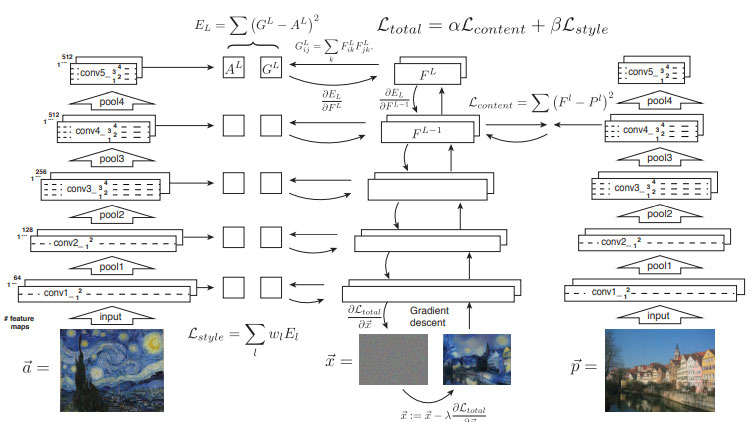
\includegraphics[width=0.7\textwidth]{style_transfer_algorithm}
	}
\end{figure}

\subsection{Feed-forward Generation Networks}
To improve the performance, Ulyanov et al. \cite{Ulyanov2016} suggest using a feed-forward generation network instead of reconstruction.
Reconstruction requires an iterative process to change the pixel values to match the desired statistics.
A feed-forward network can do this in a single evaluation.
To train such a network, they use a pre-trained network for image classification, and calculate a texture and content loss by extracting the features similar to \cite{Gatys2016}.
Johnson et al. \cite{Johnson2016} propose an almost identical framework independently.
The work of Ulyanov et al. did increase the performance, but at the expense of quality, therefor they suggest further improvements to their network \cite{Ulyanov2017}.
First, they replace \gls{BN} \cite{Ioffe2015} with \gls{IN} which alone has a significant impact on quality as can be seen in \ref{fig:style_transfer_ulyanov_BN_IN_comparison}.
Second, they teach the generator to sample from the Julesz ensemble \cite{Zhu2000} which improves variation in the outputs.
\\

\begin{figure}[h]
	\centering
	\subcaptionbox{Content Image \label{fig:style_transfer_ulyanov_content}}[0.18\textwidth]{%
		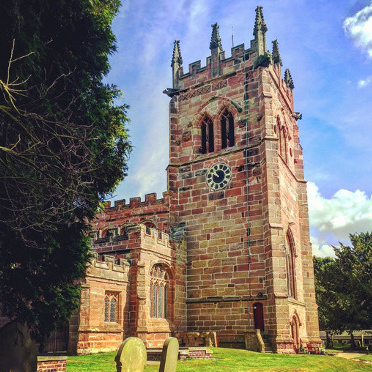
\includegraphics[width=0.18\textwidth]{style_transfer_ulyanov_content_2}\\
		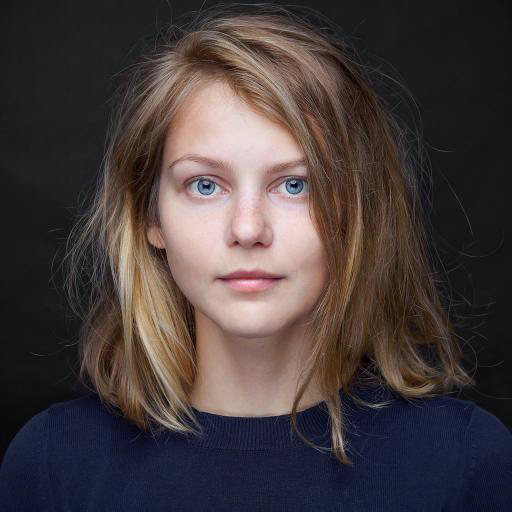
\includegraphics[width=0.18\textwidth]{style_transfer_ulyanov_content}%
	}
	\subcaptionbox{Style Image \label{fig:style_transfer_ulyanov_style}}[0.18\textwidth]{%
		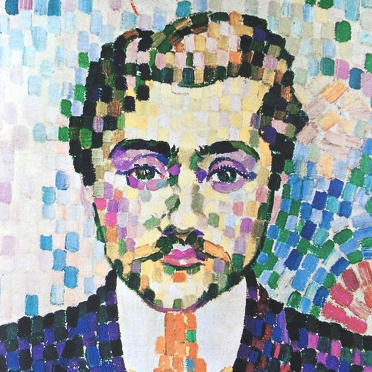
\includegraphics[width=0.18\textwidth]{style_transfer_ulyanov_style_2}\\
		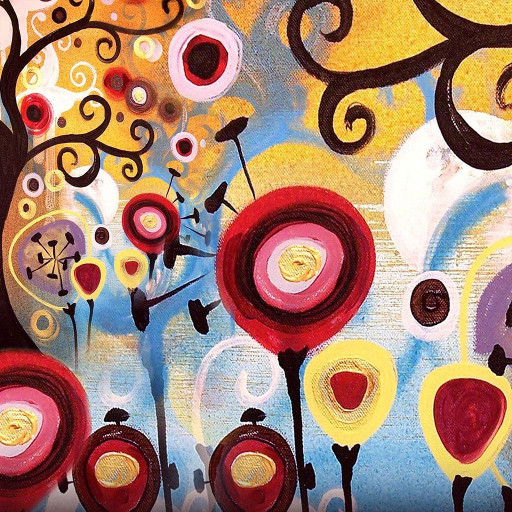
\includegraphics[width=0.18\textwidth]{style_transfer_ulyanov_style}%
	}
	\subcaptionbox{StyleNet with BN \label{fig:style_transfer_ulyanov_BN}}[0.18\textwidth]{%
		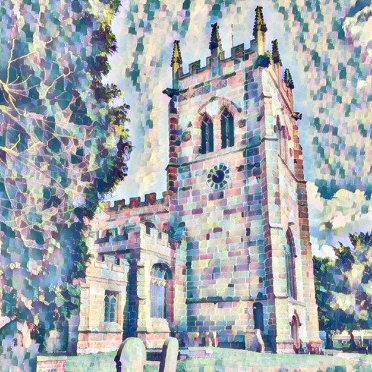
\includegraphics[width=0.18\textwidth]{style_transfer_ulyanov_BN_2}\\
		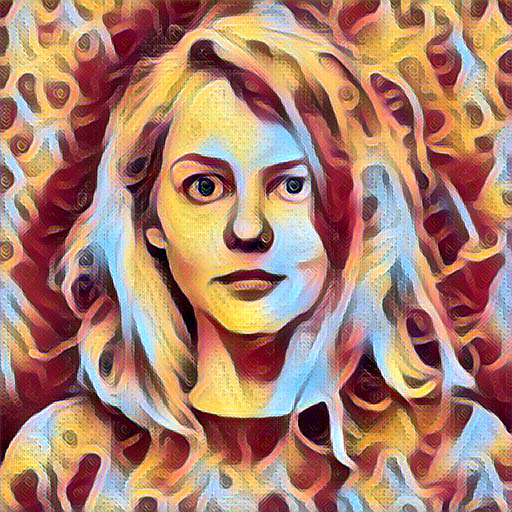
\includegraphics[width=0.18\textwidth]{style_transfer_ulyanov_BN}%
	}
	\subcaptionbox{StyleNet with IN \label{fig:style_transfer_ulyanov_IN}}[0.18\textwidth]{%
		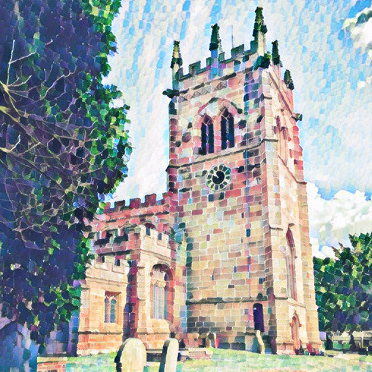
\includegraphics[width=0.18\textwidth]{style_transfer_ulyanov_IN_2}\\
		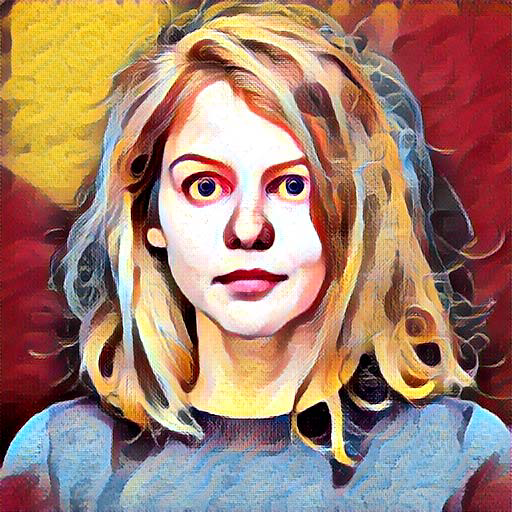
\includegraphics[width=0.18\textwidth]{style_transfer_ulyanov_IN}%
	}
	\caption{A comparison between (c) BN and (d) IN.\cite{Ulyanov2017}}
	\label{fig:style_transfer_ulyanov_BN_IN_comparison}
\end{figure}

Dumoulin et al. \cite{Dumoulin2016} observe that previous feed-forward networks are limited to one style.
In order to facilitate many different styles, there would need to be a network trained separately for each which limits the applications for mobile devices.
In order to make the network more memory efficient, they propose a conditional style transfer network; given a content image and a style name, it transforms the image to the corresponding style.
They argue that after normalization each style can be distinguished by specializing scaling and shifting parameters.
They call this \gls{CIN}.
Since it only changes the scale and shift parameters for different styles, the network requires fewer parameters.
Of the 1.6M parameters, only 3K are needed for the different styles.
Another network that puts a focus on multiple styles comes from Chen et al. \cite{Chen2017c}.
They propose a StyleBank which can store multiple convolution filter banks each representing a different style.
They use an autoencoder with in between the encoder and decoder a StyleBank layer.
During training, for each $T+1$ iterations the entire network is first trained with a perception loss for the first $T$ iterations.
Then only the autoencoder network is trained with a \gls{MSE} loss.
This way the autoencoder only retains the content and the StyleBank layer only the different styles.
This also allows them to lock the encoder and decoder to learn a new style afterwards.
While \gls{CIN} allows for multiple styles, it's still limited to the ones that were seen during training.
Huang et al. \cite{Huang2017} try to remedy this by introducing an \gls{AdaIN} layer.
Unlike the other normalization techniques, \gls{AdaIN} does not have affine parameters, and will adaptively compute these from the style image.
Figure \ref{fig:adaptive_instance_normalization} shows that their network first extracts features from the content and style image using a fixed VGG-19 network as their encoder.
The AdaIN layer then performs style transfer in the feature space and with the results the decoder constructs a new image.
During training, the content loss and style loss are calculated by extracting the features using the same VGG encoder.
To make a comparison between different networks and how they deal with unseen styles, Figure \ref{fig:style_transfer_unseen_style} gives an overview.

\begin{figure}[h]
	\centering
	\captionsetup{justification=centering}
	\captionbox{
		\label{fig:adaptive_instance_normalization}
		Adaptive Instance Normalization network by Huang et al. \cite{Huang2017}. \\
	}{
		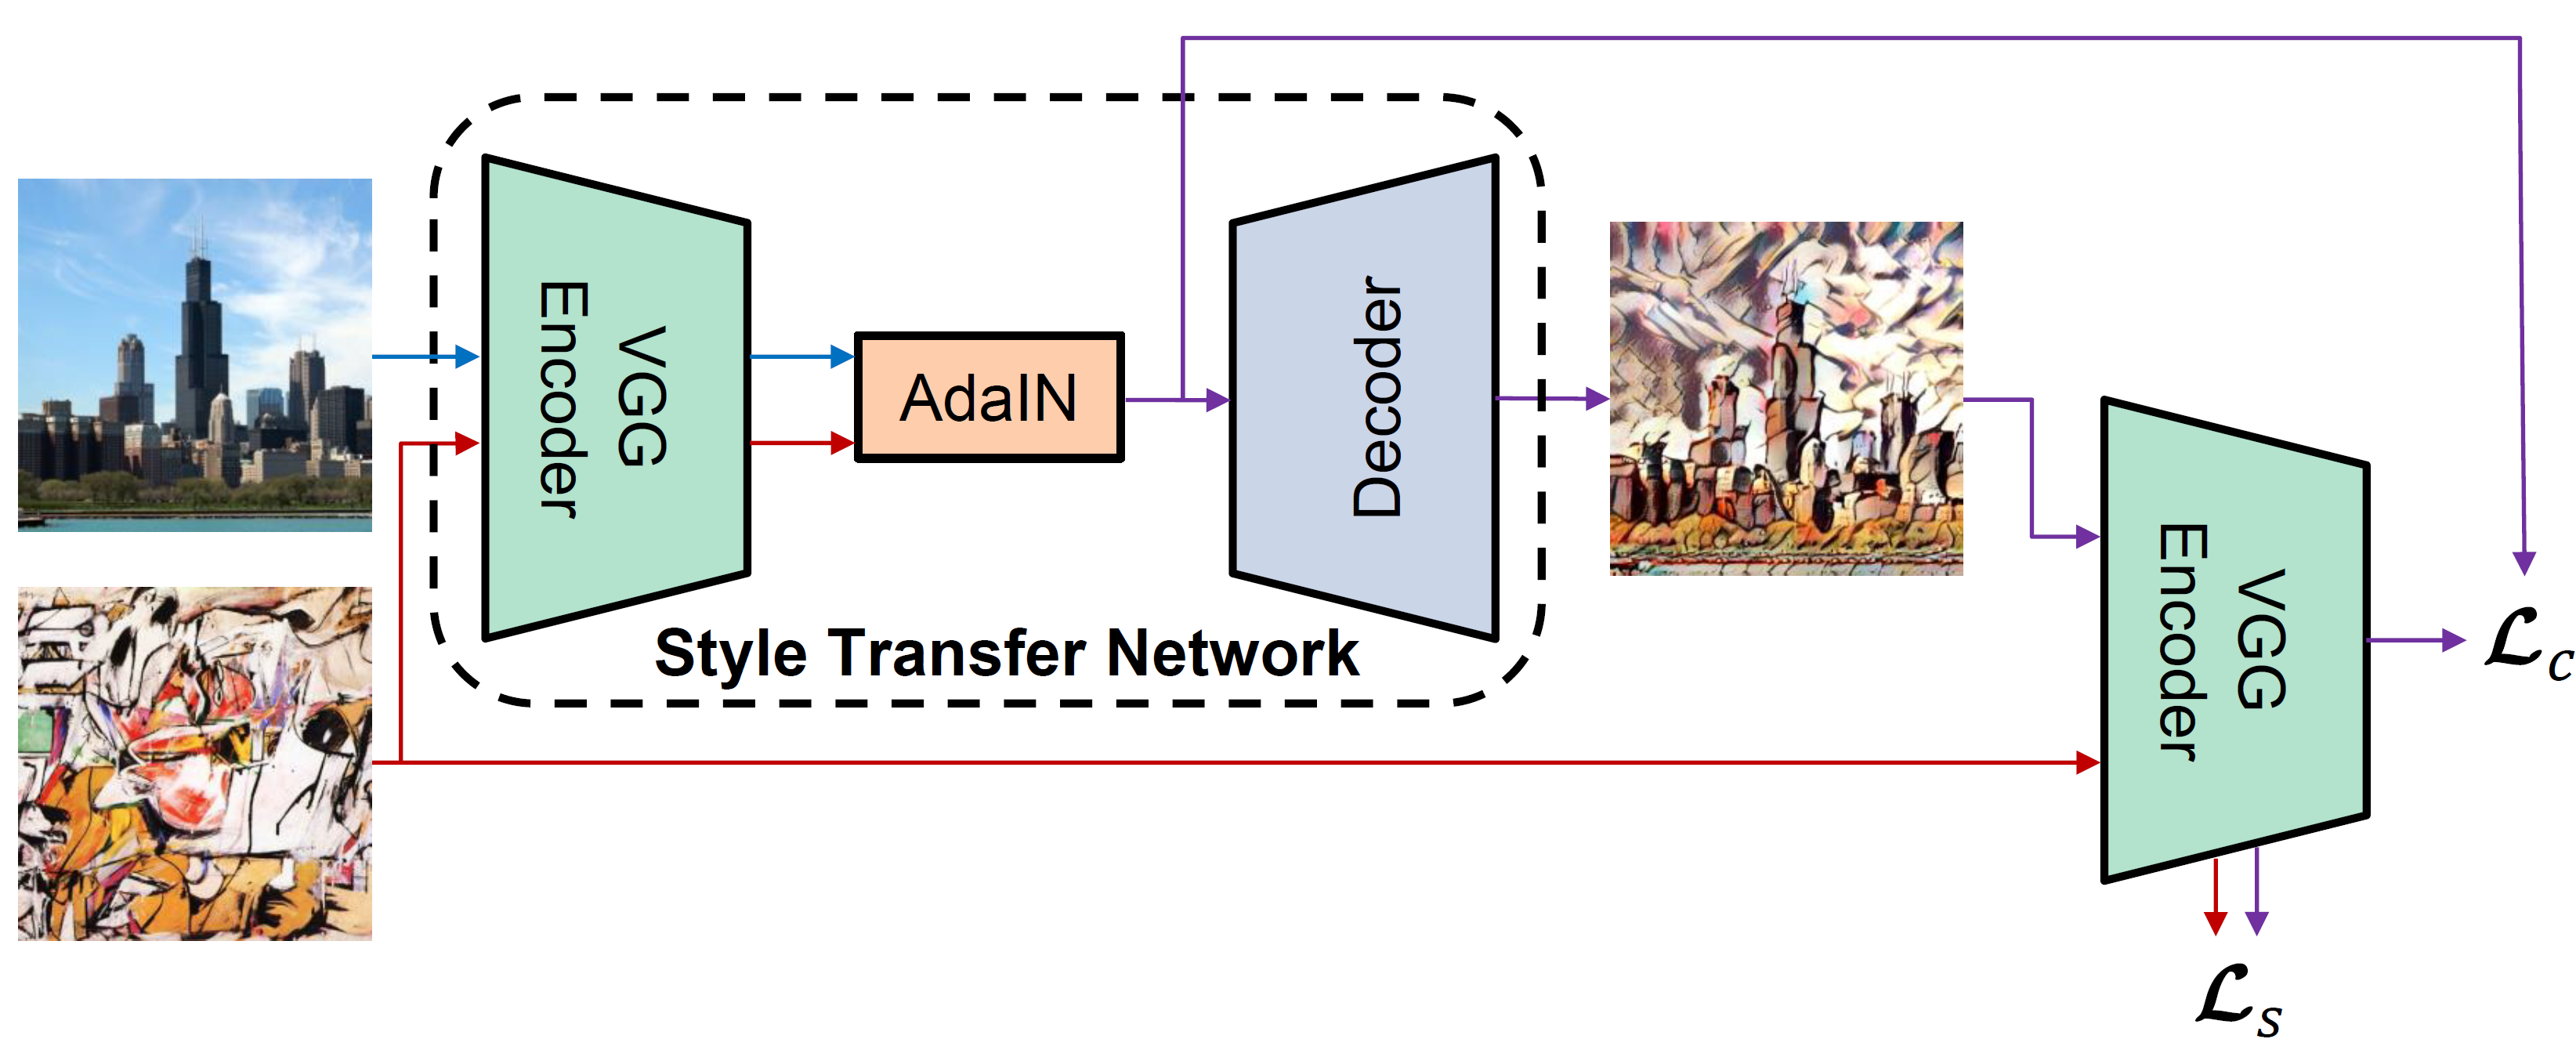
\includegraphics[width=0.8\textwidth]{adaptive_instance_normalization}
	}
\end{figure}

\begin{figure}
	\centering
	\subcaptionbox{Content Image}[0.19\textwidth]{
		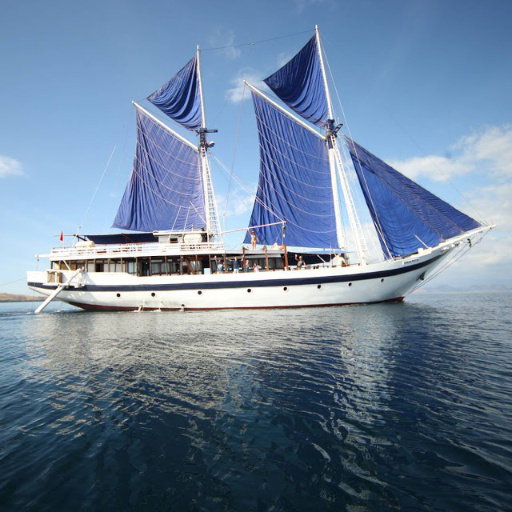
\includegraphics[width=0.19\textwidth]{style_transfer_content_a}\\
		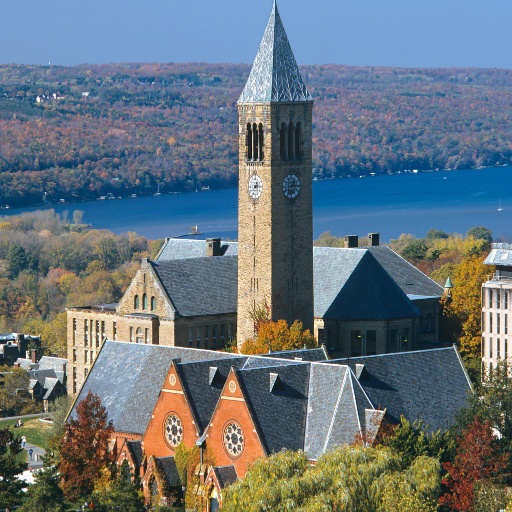
\includegraphics[width=0.19\textwidth]{style_transfer_content_b}\\
		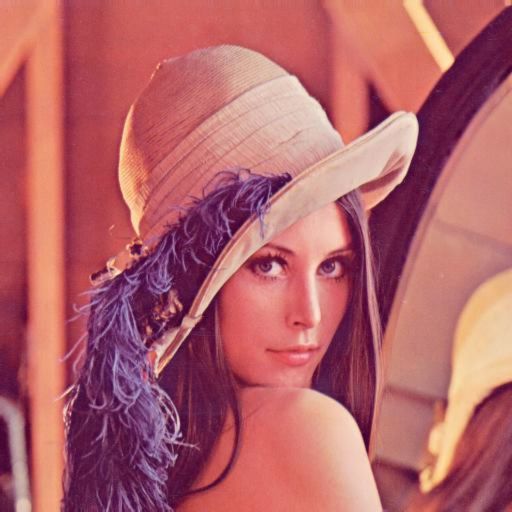
\includegraphics[width=0.19\textwidth]{style_transfer_content_c}\\
		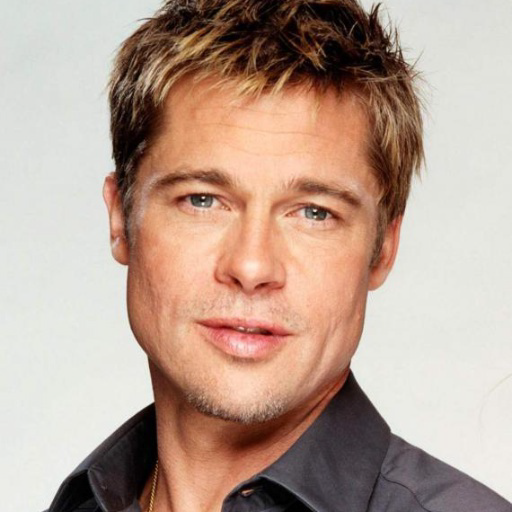
\includegraphics[width=0.19\textwidth]{style_transfer_content_d}\\
		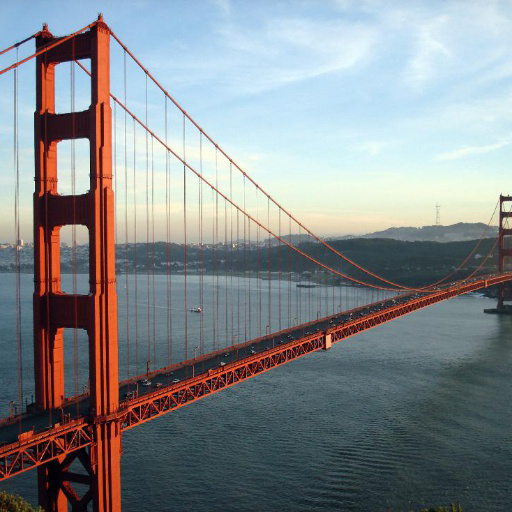
\includegraphics[width=0.19\textwidth]{style_transfer_content_e}\\
	}
	\subcaptionbox{Style Image}[0.19\textwidth]{
		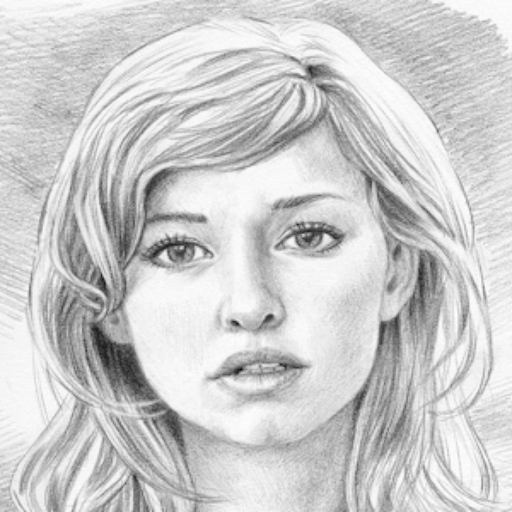
\includegraphics[width=0.19\textwidth]{style_transfer_style_a}\\
		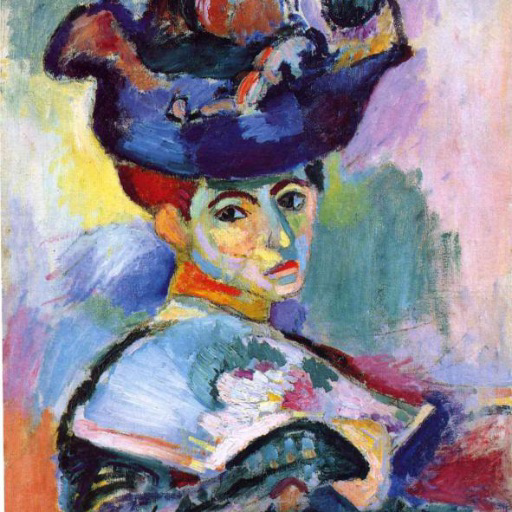
\includegraphics[width=0.19\textwidth]{style_transfer_style_b}\\
		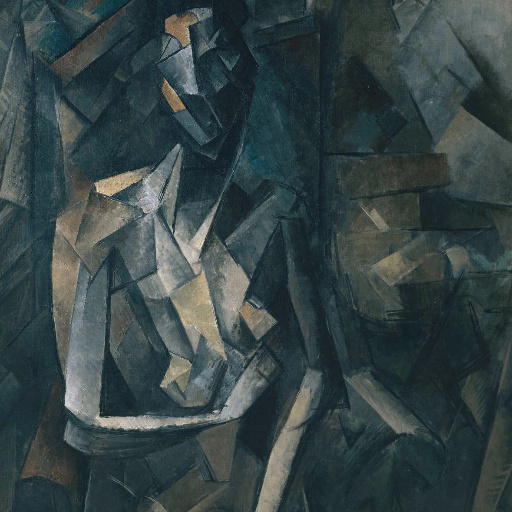
\includegraphics[width=0.19\textwidth]{style_transfer_style_c}\\
		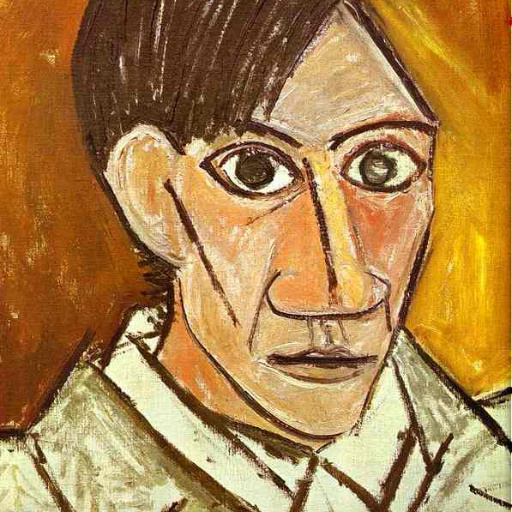
\includegraphics[width=0.19\textwidth]{style_transfer_style_d}\\
		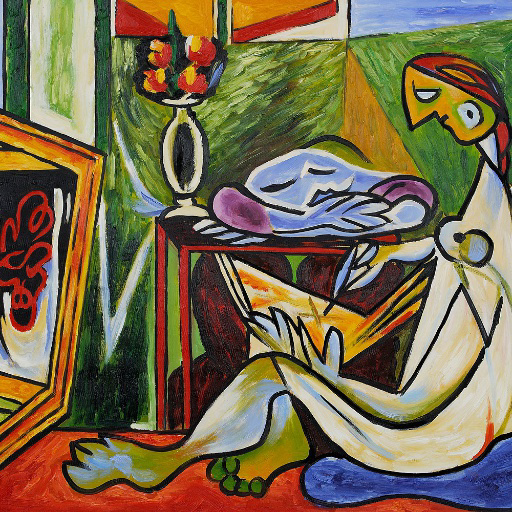
\includegraphics[width=0.19\textwidth]{style_transfer_style_e}\\
	}
	\subcaptionbox{Huang et al.}[0.19\textwidth]{
		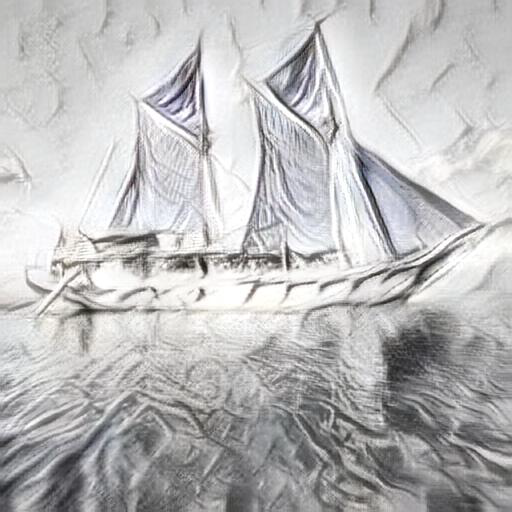
\includegraphics[width=0.19\textwidth]{style_transfer_huang_a}\\
		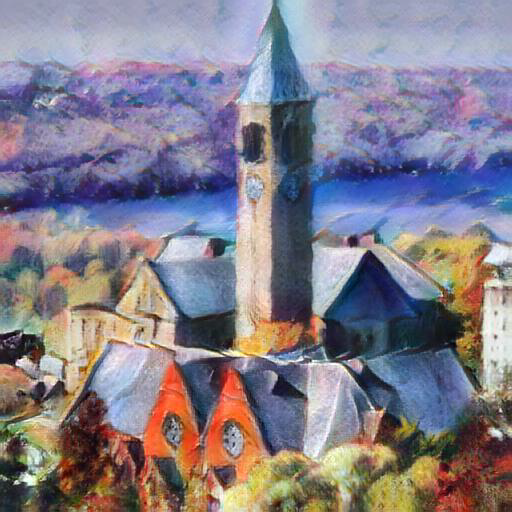
\includegraphics[width=0.19\textwidth]{style_transfer_huang_b}\\
		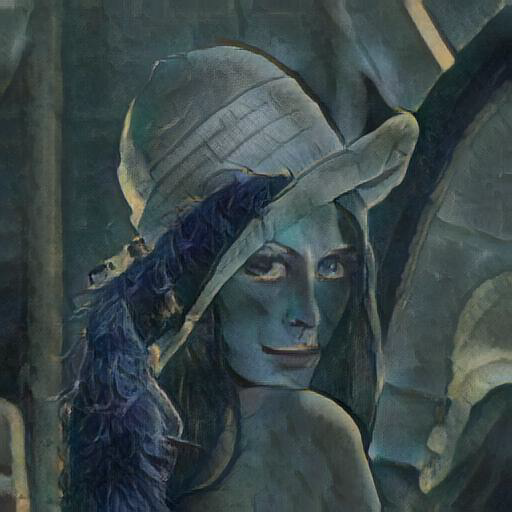
\includegraphics[width=0.19\textwidth]{style_transfer_huang_c}\\
		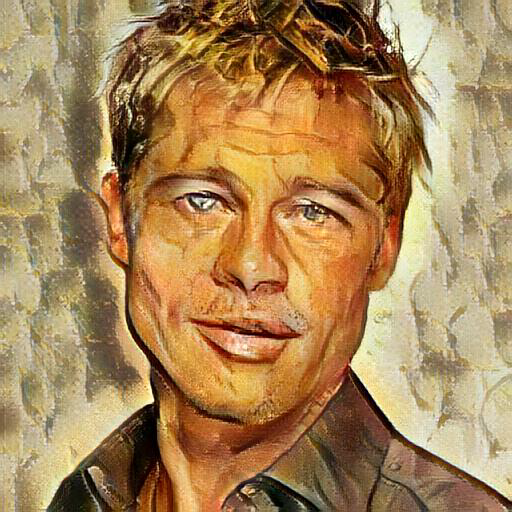
\includegraphics[width=0.19\textwidth]{style_transfer_huang_d}\\
		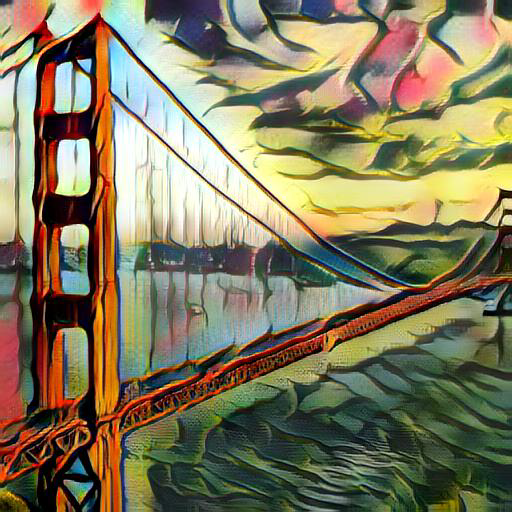
\includegraphics[width=0.19\textwidth]{style_transfer_huang_e}\\
	}
	\subcaptionbox{Ulyanov et al.}[0.19\textwidth]{
		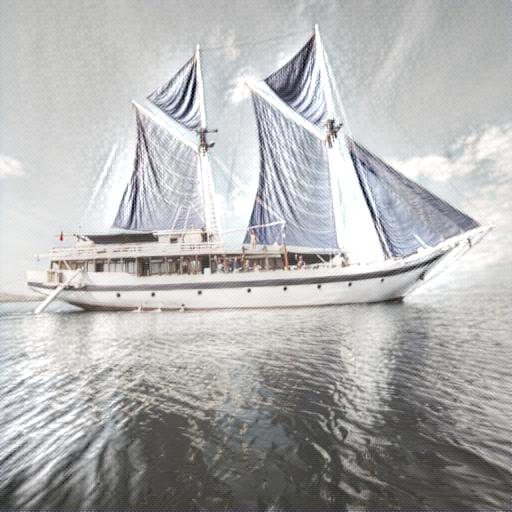
\includegraphics[width=0.19\textwidth]{style_transfer_ulyanov_a}\\
		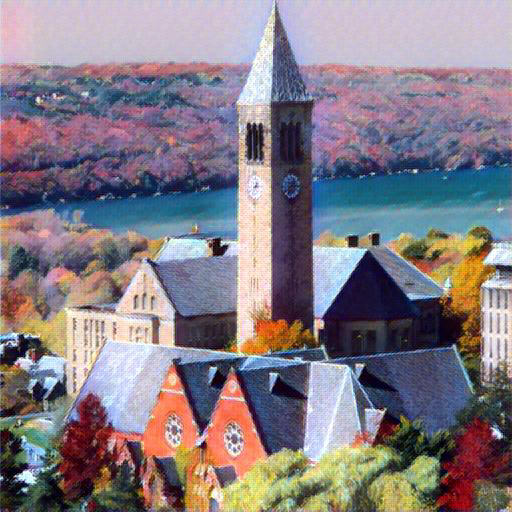
\includegraphics[width=0.19\textwidth]{style_transfer_ulyanov_b}\\
		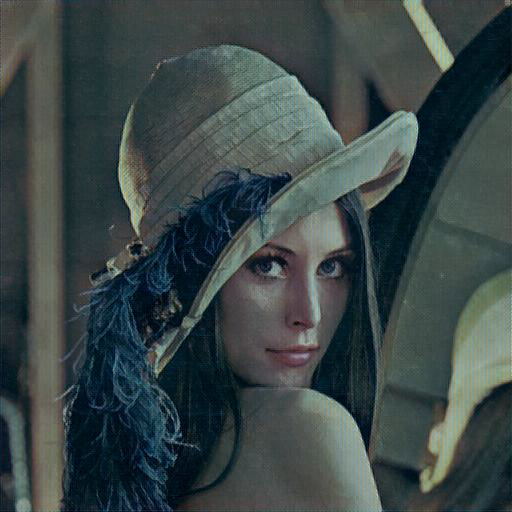
\includegraphics[width=0.19\textwidth]{style_transfer_ulyanov_c}\\
		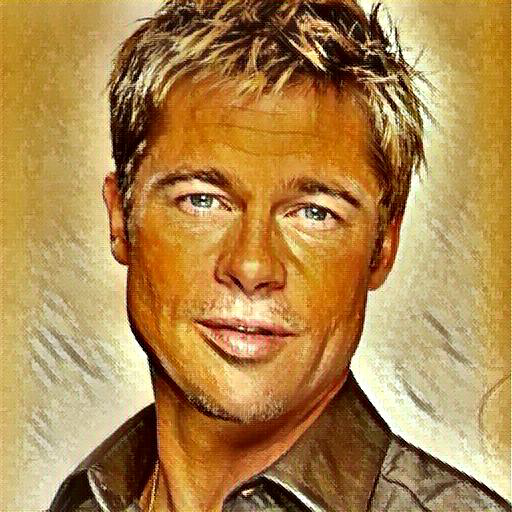
\includegraphics[width=0.19\textwidth]{style_transfer_ulyanov_d}\\
		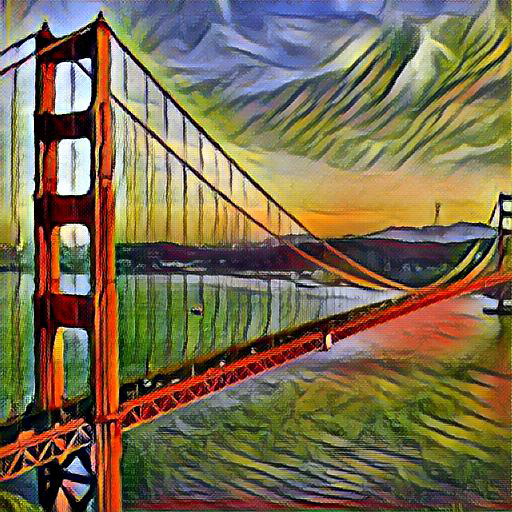
\includegraphics[width=0.19\textwidth]{style_transfer_ulyanov_e}\\
	}
	\subcaptionbox{Gatys et al.}[0.19\textwidth]{
		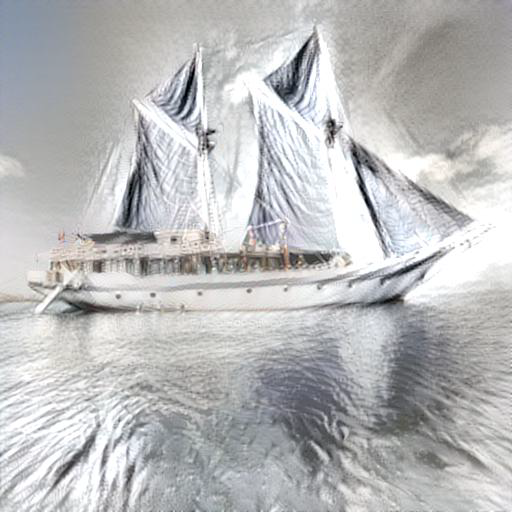
\includegraphics[width=0.19\textwidth]{style_transfer_gatys_a}\\
		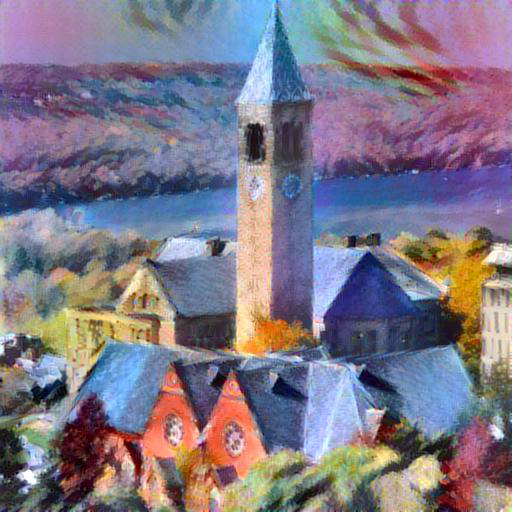
\includegraphics[width=0.19\textwidth]{style_transfer_gatys_b}\\
		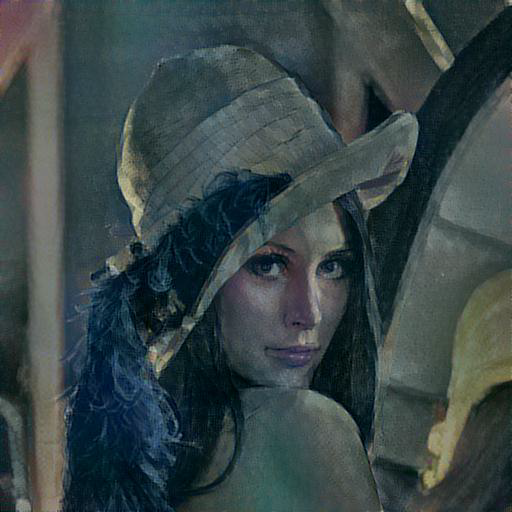
\includegraphics[width=0.19\textwidth]{style_transfer_gatys_c}\\
		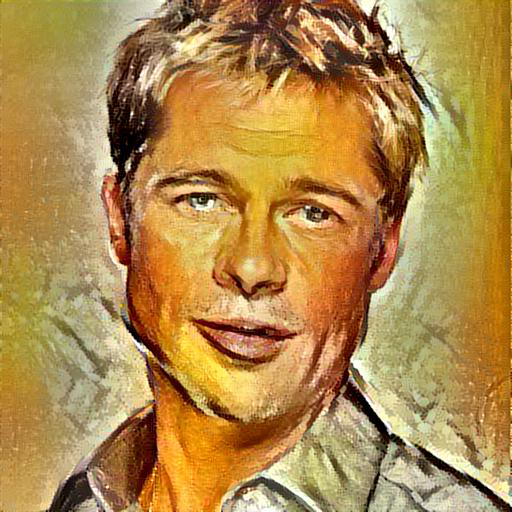
\includegraphics[width=0.19\textwidth]{style_transfer_gatys_d}\\
		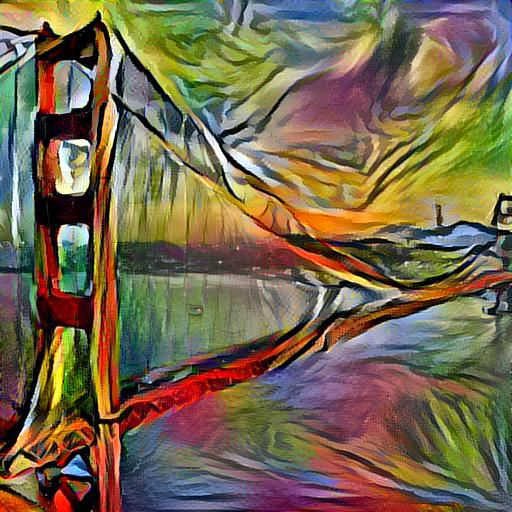
\includegraphics[width=0.19\textwidth]{style_transfer_gatys_e}\\
	}
	\caption{A comparison between different style transfers where the style was not seen during training.}
	\label{fig:style_transfer_unseen_style}
\end{figure}

\subsection{Generative Adversarial Networks}
With the introduction of \glspl{GAN}, the quality of generative models has greatly increased.
It is not surprising then that this got picked up in \gls{NST} research.
Among the first are Isola et al. \cite{Isola2016}, who use \gls{cGAN}.
They use the network from \cite{radford2016}, that uses modules of the form convolution-BatchNorm-ReLu\cite{Ioffe2015}.
Additionally, in order to pass shared features in the generator they add skip connections like with "U-Net" \cite{Ronneberger2015}.
For the discriminator, which they call PatchGAN, they validate $N\times N$ patches and take the average as output.
They take this loss together with the $L1$ loss because $L2$ loss produces blurry results.
However, this method still requires paired training samples.
Meanwhile, Taigman et al. \cite{Taigman2016} are doing research in unsupervised domain transfer.
Research in domain transfer can be easily adjusted for use in \gls{NST}, but this is not possible the other way around.
Their network uses an autoencoder as the generator and they assume that the encoder is fixed between domains.
The discriminator has a ternary output and distinguishes between real, fake and reconstruction.
They add several new loss functions which check the consistency between the two domains (consistency loss) and whether $G$ performs perfect reconstruction (reconstruction loss).
For the encoder, they use a pre-trained network that is trained on paired samples though.
In order to make the network completely unsupervised, Yi et al.\cite{Yi2017} propose DualGAN, Kim et al. \cite{Kim2017} DiscoGAN and Zhu et al. \cite{Zhu2017b} CycleGAN, which are all three essentially the same proposal.
The entire model consists of two cycle-consistent networks where each translates from one domain to the other.
A cycle-consistent network will first translate the input to a target domain and then back to the original domain.
Each domain has a discriminator which compares the real input from one network with the fake from the other; the adversarial loss.
In addition to this there's a cycle-consistency loss, which is the \gls{MSE} between the input and the reconstructed image as you can see in Figure \ref{fig:style_transfer_algorithm_cyclegan}.
The goal is to minimize the adversarial and cycle-consistency loss, while maximizing the discriminators' accuracy.

\begin{figure}[h]
	\centering
	\captionbox{
		\label{fig:style_transfer_algorithm_cyclegan}
		The cycle-consistent network by Zhu et al. \cite{Zhu2017b}.
		Unsupervised image-to-image translation between domains $X$ and $Y$ is established by training the generators $G$, $F$ and discriminators $D_X$, $D_Y$.
		During training cycle-consistency loss is calculated under the assumption that $F(G(x))\shouldeq x$ and $G(F(y))\shouldeq y$.
	}{	
		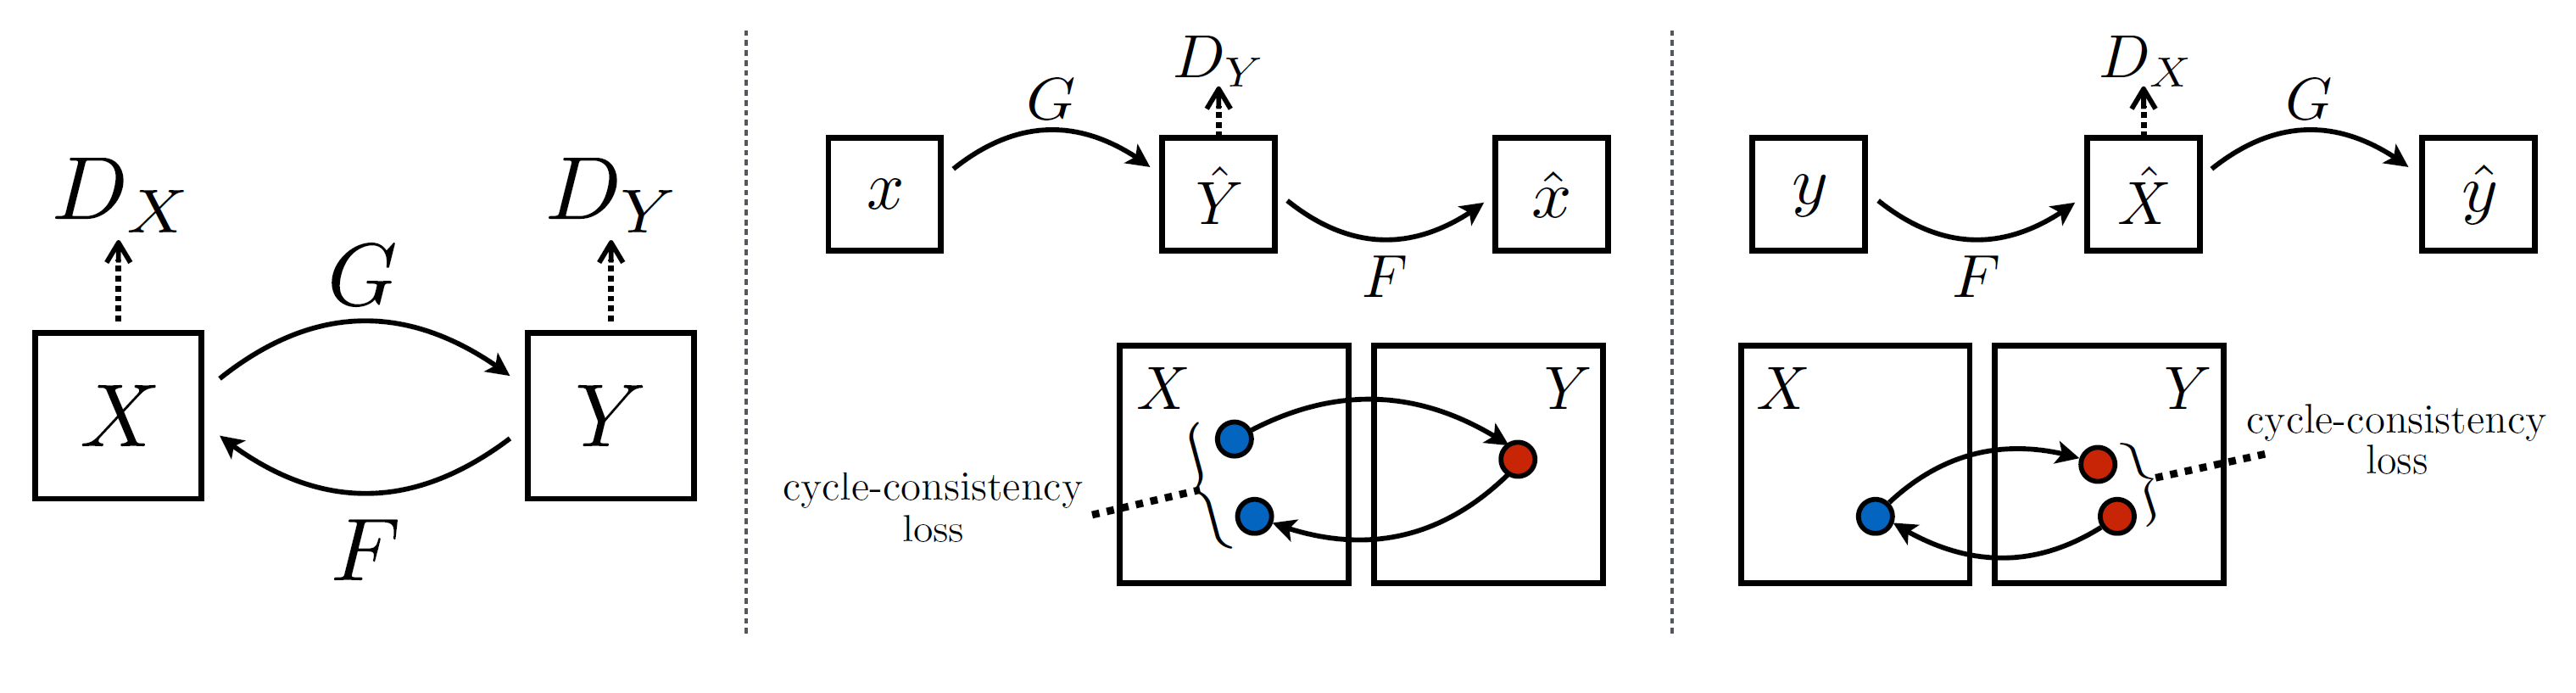
\includegraphics[width=\textwidth]{style_transfer_algorithm_cyclegan}%
	}
\end{figure}

Zhu et al. \cite{Zhu2017b} also introduce an identity loss.
Liu et al. \cite{Liu2017} introduce the latent space concept which assumes that paired images from different domains can be mapped to a shared latent space with the same latent representation.
Their network consists of two domain image encoders $E\textsubscript{$1$}$ and $E\textsubscript{$2$}$, two domain image generators $G\textsubscript{$1$}$ and $G\textsubscript{$2$}$, and two domain discriminators $D\textsubscript{$1$}$ and $D\textsubscript{$2$}$, as can be seen in \ref{fig:style_transfer_algorithm_unit}.
The encoders and generators are paired and form a \gls{VAE} \cite{kingma2022}.
The encoder maps the input to latent space, and the generator reconstructs the image.
This is the reconstruction loss.
They use weight-sharing, which shares the weight of the last two layers of the encoders and of the first two layers of the generators.
The generators and discriminators are paired to form a \gls{GAN}.
The generator can also construct an image from the latent code from the other encoder's input.
This image is used to train the \gls{GAN}.
They also show that the shared-latent space assumption implies cycle-consistency, which is the final loss function of the network.

\begin{figure}
	\centering
	\captionbox{
		\label{fig:style_transfer_algorithm_unit}
		Liu et al. \cite{Liu2017}.
	}{	
		\subcaptionbox{The shared latent space assumption.}[0.34\textwidth]{%
			\includegraphics[width=0.34\textwidth]{style_transfer_algorithm_unit_a}%
		}
		\subcaptionbox{The unsupervised image-to-image translation network.}[0.64\textwidth]{%
			\includegraphics[width=0.64\textwidth]{style_transfer_algorithm_unit_b}%
		}
	}
\end{figure}

\subsection{Evaluation Metric}
\label{sec:style_transfer_metrics}
There are several methods to evaluate the quality of a generated image. 
A first metric is through human evaluation, where a score is given based on generation quality.
This proved to be inconsistent as a person's perception can change over time.
Afterwards, new metrics were introduced which will be discussed here. \cite{Hoyez2022}

\begin{enumerate}
	\item \textbf{\gls{PD}} is proposed by Johnson et al. \cite{Johnson2016}.
	It uses the VGG-16 network \cite{Simonyan2015} trained on ImageNet \cite{Deng2009} to define perceptual loss functions.
	These are extracted from the layers for the style and content images, and compared to the generated image.
	The lower the score, the better.
	\item \textbf{\gls{IS}}, as described by Salimans et al. \cite{Salimans2016}, uses a pre-trained Inception model \cite{Szegedy2015} to describe the quality of the generated images.
	It prescribes that the entropy of the distribution of predicted labels for individual images needs to be minimized while the entropy of the distribution across all images need to be high.
	This equates to each image having generated a distinct label and the labels being equally distributed.
	The closer to 1, the better.
	\item \textbf{\gls{FID}} is the most used measurement and suggested by Heusel et al. \cite{Heusel2017} to enhance \gls{IS}, because it is only calculated on the distribution of the generated images.
	\gls{FID} uses the Gaussian distribution of both real and generated images as it calculates the Fréchet distance \cite{Frechet1957} between them.
	The Gaussians are formed from the coding layer of the Inception network \cite{Szegedy2015}.
	The lower, the better.
	\item \textbf{\gls{LPIPS}} is a metric developed by Zhang et al. \cite{Zhang2018} and the second most popular.
	It calculates the distance between the activations of the hidden layers in an object detection model (several models are proposed).
	They show that this correlates closely to human perception.
	It can also be used to evaluate the diversity of a network by calculating the average \gls{LPIPS} score of a pair of randomly generated outputs.
	The higher, the better.
\end{enumerate}

\subsubsection{Summary}
There are plenty of other evaluation metrics available that also try to correlate closely to human evaluation, but they are mostly just attempts to improve previously discussed metrics.
Until this day, image similarity metrics continue to be a challenging problem.

\section{Content Based Image Retrieval}
\gls{CBIR}, a long-established research area, is the task of finding semantically matching or similar content images for a specified query image.
This has become increasingly relevant with the exponential growth of image and video data and the need to effectively search these image collections.
\gls{CBIR} has been used specifically for person re-identification, remote sensing, medical image search, and shopping recommendations in online marketplaces, among many others \cite{Chen2021a}.
Image retrieval can be categorized into two different groups: \gls{CIR} and \gls{IIR}.
\gls{CIR}'s goal is to find images within the same category as the query, while \gls{IIR} tries to find images with a particular instance given in the query image.
The general workflow of \gls{CBIR} is illustrated in \ref{fig:image_retrieval_flowchart}.
This thesis will only discuss query formation, image representation, image scoring, and search re-ranking.

\begin{figure}
	\centering
	\includegraphics[width=0.65\textwidth]{image_retrieval_flowchart}%
	\label{fig:image_retrieval_flowchart}
	\caption{
		The general workflow of Content Based Image Retrieval. \cite{Zhou2017}
	}
\end{figure}

\textbf{Query Formation} can be done several ways.
A user might want to find images based on keywords, which is your standard classification task.
Instead of just giving a series of keywords, these can also be arranged in a layout.
A query by concept layout will then search for an image with the same arrangement \cite{Xu2010}.
Similarly, a query by color layout will search for that arrangement of colors in the images \cite{Wang2011}.
It's also possible that a user wants to find images similar to a sketch (query by sketch) \cite{Cao2010} or another image (query by example) \cite{Radenovic2017}.
An overview can be found in Fig. \ref{fig:image_retrieval_query_formation}.

\begin{figure}[h]
	\centering
	\includegraphics[width=0.7\textwidth]{image_retrieval_query_formation}%
	\caption{
		An overview of the different kinds of queries with corresponding retrieval results. \cite{Zhou2017}
	}
	\label{fig:image_retrieval_query_formation}
\end{figure}

\textbf{Image Representation} is a major challenge with image retrieval.
It's goal is to proficiently measure similarity between images.
Clearly, directly comparing pixels values is impracticable, so methods that extract visual features from images are used.
They are transformed into a fixed-sized vector which form a representation of the image.
Before deep learning, hand crafted feature algorithms were used.
From these, \gls{SIFT} \cite{Lowe1999} was the most popular.
Thousands of features can be extracted this way, which is too much for an efficient query response.
These features are further compressed for which various methods exist, called feature aggregation.

\textbf{Image scoring} gives the results during a search a relevance score for ranking.
This score is determined by one of two ways:
During feature aggregation, the image is represented with a fixed-sized vector.
The relevance can be calculated with the $L_p$-normalized distance between the feature aggregation vectors.
Scoring can also be quantified based on voting.
This can be achieved by counting each similar feature to the vote \cite{Zhou2011}, or through the calculation of \gls{TF-IDF} \cite{Zhang2011}.

\textbf{Search Reranking} are post-processing techniques that improve the accuracy of the query.
Among them is geometric context verification, which will try to eliminate false similarities by looking at geometric context, like rotation, scale and the relations between local features.
Another is to reuse the highest ranked results to create new queries which can expand on the original.
Missed features in the original query can be found this way and improve recall performance.
As a last improvement, different retrieval techniques can be merged together to give better results with retrieval fusion.

The model used in this work, by Radenovic et al. \cite{Radenovic2017}, trains a VGG network from reconstructed 3D models obtained by retrieval and structure-from-motion methods.
This allows them to use the geometry and camera positions to enhance the feature extraction along with several other optimization techniques.
During training, they make use of the contrastive loss.
Contrastive loss is minimized when similar image pairs are close to each other in embedding space and different pairs are far away.

\section{Deep learning in the Art domain}
\label{sec:related_papers}
Various papers have already discussed different techniques to improve object detection and pose estimation on artworks.
In this section, three of those papers will be discussed.
One paper discusses how the digitization of artworks can benefit the analysis of art collections.
The other two discuss techniques of how existing models can be adapted to work on art collections.
\\

Through digitization, analysis of art collections has become more efficient.
Artists are constantly inspiring and being inspired, and in order to correctly analyze the relation between paintings and artists, it's beneficial to have a method that finds their inspirations.
One way that can be achieved is by using image retrieval, which gives good results, but only when the works are visually similar, like with religious paintings.
In other cases, the inspiration is drawn from themes, which involve composition, lighting and poses.
Jenicek et al. \cite{Jenicek2019} propose finding these relations by analyzing the similarity between poses.
From a database of images the poses are estimated and normalized.
They then employ a two step process: with a query image and fast matching, they generate a shortlist of possible hits.
Afterwards, geometric validation filters out impossible alignments with the query image.
Their experiments show significant improvements over previous methods.
They also note some failure cases where pose estimation falls short, like failing to find keypoints or making associations with wrong poses.
\\
\\

\begin{figure}[h]
	\centering
	\captionbox{
		\label{fig:related_papers_madhu}
		Improvements to the state-of-the-art by Madhu et al. \cite{Madhu2020}.
	}{	
		\subcaptionbox{Original}[0.20\textwidth]{%
			\includegraphics[width=0.20\textwidth]{related_papers_vase}%
		}
		\subcaptionbox{OpenPose}[0.20\textwidth]{%
			\includegraphics[width=0.20\textwidth]{related_papers_vase_sota}%
		}
		\subcaptionbox{Madhu et al.}[0.20\textwidth]{%
			\includegraphics[width=0.20\textwidth]{related_papers_vase_stl}%
		}
	}
\end{figure}

To improve these shortcomings on Greek vases, Madhu et al. \cite{Madhu2020} apply style transfer to the COCO dataset with AdaIN in the style of those vases and use this for fine-tuning.
They use a top-down architecture with Faster R-CNN as detector and HRNet for pose estimation.
They also created their own small dataset to evaluate their improvements (Figure \ref{fig:related_papers_madhu}).
Kadish et al. \cite{Kadish2021} have the same idea and also use AdaIN to stylize the COCO dataset.
They randomly sample artworks from the Painter by Numbers dataset from Kaggle \cite{PainterByNumbers} for the style images and using it to fine-tune the Faster R-CNN network for object detection.
Both papers found an improvement in the performance of the networks on art collections, which is further discussed in Section \ref{sec:improvements_related_papers}.
\\

Part of this thesis will combine the previously discussed work.
While Madhu et al. only fine-tuned a network to work better for Greek vases, it would be more useful if the fine-tuned model could be used more generally.
This is what Kadish et al. achieve, but they focused on the object detection task.
Here, both methods will be combined to achieve improvements in pose estimation on non-specific art collections.
\chapter{Titel tweede hoofdstuk}
\label{chap:evaluation}

Vul aan.

\lipsum[9-10]

\section{Sectie titel}
\label{sec:scalable_faafo}

Vul aan.

\lipsum[10-12]
Voorbeeld figuur.
\chapter{Improving Pose Estimation with Style Transfer}
\label{chap:improvements}
Having established a baseline, it is now possible to search for improvements.
In this chapter, 2 techniques will be explored to see if they can improve \gls{HPE}.
Using the same algorithms as seen in the previous chapter, they will now be used to:
(1) transform an input artistic image to a photographic image to estimate poses on or
(2) be trained with a dataset that is augmented with images that are transformed to different styles.

\section{Pose Estimation after Style Transform}
\label{chap:improvements_style_transfer}
One option to predict poses on an artwork is to transform it first to photographic realism and let the plain model run on it.
As previously seen in section \ref{baseline_human_art_results}, the results on photographs are dramatically better.
If artworks are successfully transformed to that style, there is no need to train a new model and the extensive amount of datasets created for this task are available.
To validate this, SWAHR and ViTPose are run on the Human-Art dataset after it was transformed using AdaIN and CycleGAN.
For CycleGAN, 3 styles are used to perform this task, namely baroque, impressionism and renaissance.
AdaIN uses 3 style images for each style previously mentioned.
Fig. \ref{fig:baseline_pose_estimation_evalutaion} shows the selection made for this.
Before transforming the artwork, the size is checked and resized to 1024 if either of the sides is bigger than that, and only then.
This is done because some artworks in the dataset are quite large and cause Out-Of-Memory errors.
Otherwise, no other distortions are applied.
This adds the total number of tests to be up to 24.

\subsection{Results}
\label{chap:improvements_results_style_transfer}
As seen in section \ref{baseline_results_coco_style_transfer}, here as well, style transfer is only more detrimental to the results.
As seen in Table \ref{tab:experiments_pose_estimation_after_style_transfer}, the same observations can be made: Only ViTPose scores, but with very low precision and high recall.

\begin{table*}
    \setlength\tabcolsep{4pt}
    \caption{Performance of plain Pose Estimation models after Artwork is transformed with different Style Transfer models. }
    \centering
    \footnotesize
    \label{tab:experiments_pose_estimation_after_style_transfer}
    \begin{tabular}{ l|ccccc|ccccc }
        \hline
        \bf{Method}&\bf{AP}&\bf{AP$^{50}$}&\bf{AP$^{75}$}&\bf{AP$^{M}$}&\bf{AP$^{L}$}&\bf{AR}&\bf{AR$^{50}$}&\bf{AR$^{75}$}&\bf{AR$^{M}$}&\bf{AR$^{L}$}\cr
        \hline
        \multicolumn{11}{c}{\bf{AdaIN}}\cr
        \multicolumn{11}{c}{\bf{Trained on Baroque dataset}}\cr
        \hline
        SWAHR & 0 & 0 & 0 & 0 & 0 & 0 & 0 & 0 & 0 & \cr
        ViTPose & 0.056 & 0.109 & 0.052 & 0.002 & 0.064 & 0.463 & 0.700 & 0.486 & 0.058 & 0.501 \cr
        \hline
        \multicolumn{11}{c}{\bf{Trained on Impressionism dataset}}\cr
        \hline
        SWAHR & 0 & 0 & 0 & 0 & 0 & 0 & 0 & 0 & 0 & 0 \cr
        ViTPose & 0.044 & 0.089 & 0.043 & 0.002 & 0.051 & 0.406 & 0.648 & 0.427 & 0.051 & 0.439 \cr
        \hline
        \multicolumn{11}{c}{\bf{Trained on Renaissance dataset}}\cr
        \hline
        SWAHR & 0 & 0 & 0 & 0 & 0 & 0 & 0 & 0 & 0 & 0 \cr
        ViTPose & 0.052 & 0.100 & 0.047 & 0.001 & 0.058 & 0.441 & 0.0679 & 0.457 & 0.045 & 0.477 \cr
        \hline
        \multicolumn{11}{c}{\bf{CycleGAN}}\cr
        \multicolumn{11}{c}{\bf{Trained on Baroque dataset}}\cr
        \hline
        SWAHR & 0 & 0 & 0 & 0 & 0 & 0 & 0 & 0 & 0 & 0 \cr
        ViTPose & 0.068 & 0.128 & 0.066 & 0.014 & 0.075 & 0.520 & 0.768 & 0.555 & 0.195 & 0.551 \cr
        \hline
        \multicolumn{11}{c}{\bf{Trained on Impressionism dataset}}\cr
        \hline
        SWAHR & 0 & 0 & 0 & 0 & 0 & 0 & 0 & 0 & 0 & 0 \cr
        ViTPose & 0.059 & 0.113 & 0.055 & 0.020 & 0.064 & 0.470 & 0.717 & 0.488 & 0.227 & 0.493 \cr
        \hline
        \multicolumn{11}{c}{\bf{Trained on Renaissance dataset}}\cr
        \hline
        SWAHR & 0 & 0 & 0 & 0 & 0 & 0 & 0 & 0 & 0 & 0 \cr
        ViTPose & 0.057 & 0.107 & 0.052 & 0.012 & 0.062 & 0.458 & 0.694 & 0.471 & 0.183 & 0.485 \cr
        \hline
    \end{tabular}
\end{table*}

\section{Augmenting COCO Dataset for Pose Estimation Training}
\label{chap:improvements_augmentation}
The second option that's been explored is the augmentation of the dataset with styled images.
The chosen pose estimation algorithms, SWAHR and ViTPose, will be trained on several different stylized datasets.
A combination of the COCO dataset and the stylized dataset is used, and one with only the stylized dataset.
The stylized datasets are created by applying both CycleGAN and AdaIN to the COCO dataset.
One with a mixture of the baroque, impressionism and renaissance models, and one with only the impressionism model.
This results in a combination of 18 models.
The experiments will be conducted on the COCO-dataset as well as the Human-Art dataset.
While the problem specifically tries to improve the performance on artworks, it's still interesting to also validate the results on the COCO-dataset.


\subsection{Creation of datasets}
\label{sec:improvements_dataset_pose_estimation}
For each augmented dataset, the coco annotations file was used as template.
All metadata of the file was kept while only changing the id and file name.
To each id a number of several hundred billions was added depending on the style transfer model.
The file name points to the new location of the stylized image.
A stylized version of COCO was created from each style transfer model that CycleGAN was trained for discussed in section \ref{baseline_training_style_transfer}, except impressionism for 2000 epochs.
Other versions were created for AdaIN.
Since AdaIN requires a style image, the images used for training the CycleGAN models were used for this purpose.
The style dataset was cycled through to transform the COCO dataset with AdaIN.
The decision to not use one image as a representation for each style was made so that the dataset is more generalized.
Afterwards, a new annotation file was created from a mixture of baroque, impressionism and renaissance stylized images, and one of only the impressionism style.
For each, a version was made which is appended to the COCO dataset and one that stand on its own.
During training it was noticed that the stylized images were inverted, resulting in 2 models being trained on the inverted dataset.
These were the COCO + mixed and mixed models.

\subsection{Training}
\label{sec:improvements_training_pose_estimation}
All models are trained with the default parameters initiating the weights with the pre-trained model.
They're trained for 200 epochs and the models are saved from 100th epoch every 20 epochs.
As a control, 2 models are trained from nought, which are the inverted mixed model and the COCO + impressionism model.
These were trained for the default 300 epochs and were also saved from 100th epoch every 20 epochs.

\subsection{Results}
\label{sec:improvements_results_pose_estimation}
For the SWAHR network, shown in table \ref{tab:experiments_style_transfered_pose_estimation_coco}, the best results are found with the model trained on the COCO + AdaIN mixed style transfer dataset.
The second best network was trained on the COCO + CycleGAN mixed style transfer dataset.
For the ViTPose network, the best results are with COCO + CycleGAN mixed and COCO + CycleGAN impressionism being the second best.
For AdaIN, there's a falloff of 7 to 10\% AP between the datasets with COCO and the ones without.
For CycleGAN, this falloff is less; between 0.2 and 4\% AP.
The best precision is found using the SWAHR model, while ViTPose has the honor of having the best recall.
Table \ref{tab:experiments_style_transfered_pose_estimation_coco} compares the best models with the baseline.
It shows that the pre-trained SWAHR model has the best precision of all of the models and trained on the COCO + AdaIN Mixed style transfer dataset, SWAHR also has the second best precision.
ViTPose trained on COCO + CycleGAN mixed style transfer dataset has the best recall.
The networks trained from the ground up don't have any significant difference between the other networks.

The results on the Human-Art dataset are shown in table \ref{tab:experiments_style_transfered_pose_estimation_humanart}.
Here, one dataset takes the crown.
Both SWAHR as well as ViTPose have the best results for the models trained on the COCO + CycleGAN mixed style transfer dataset.
The second best model for SWAHR is trained on the COCO + AdaIN mixed dataset and for ViTPose this is the one trained on COCO + CycleGAN impressionism.
The falloff between the COCO and non-COCO datasets is between 5 to 9\% AP for AdaIN, and 2 to 3\% AP for CycleGAN.
The best precision and recall belongs to the SWAHR models.
Comparing the best models to the baseline, they still remain the best models overall with an increase of 3 to 5\% AP.
There's no significant difference between the non-initialized and bootstrapped networks.

\begin{table*}
    \setlength\tabcolsep{4pt}
    \vspace{0.2em}
    \caption{Performance of different Pose Estimation models trained on Style Transformed datasets on COCO dataset. }
    \begin{center}
    \footnotesize
    \label{tab:experiments_style_transfered_pose_estimation_coco}
    \begin{tabular}{ l|ccccc|ccccc }
        \hline
        \bf{Method}&\bf{AP}&\bf{AP$^{50}$}&\bf{AP$^{75}$}&\bf{AP$^{M}$}&\bf{AP$^{L}$}&\bf{AR}&\bf{AR$^{50}$}&\bf{AR$^{75}$}&\bf{AR$^{M}$}&\bf{AR$^{L}$}\cr
        \hline
        \multicolumn{11}{c}{\bf{AdaIN}}\cr
        \multicolumn{11}{c}{\bf{Trained on COCO + Mixed Style Transfer}}\cr
        \hline
        SWAHR & \bf{0.679*} & \bf{0.874*} & 0.735 & \bf{0.628*} & 0.751 & \bf{0.732} & \bf{0.902} & 0.782 & 0.651 & 0.824 \cr
        ViTPose & 0.618 & 0.859 & 0.685 & 0.599 & 0.661 & 0.748 & 0.924 & 0.816 & 0.709 & 0.805 \cr
        \hline
        \multicolumn{11}{c}{\bf{Trained on COCO + Impressionism Style Transfer}}\cr
        \hline
        SWAHR & 0.669 & 0.862 & 0.733 & 0.607 & \bf{0.755*} & 0.729 & \bf{0.902} & 0.782 & 0.651 & \bf{0.834} \cr
        ViTPose & 0.609 & 0.843 & 0.664 & 0.590 & 0.654 & 0.742 & 0.916 & 0.801 & 0.702 & 0.799 \cr
        \hline
        \multicolumn{11}{c}{\bf{Trained on Mixed Style Transfer}}\cr
        \hline
        SWAHR & 0.603 & 0.843 & 0.661 & 0.535 & 0.704 & 0.676 & 0.882 & 0.726 & 0.586 & 0.794 \cr
        ViTPose & 0.518 & 0.783 & 0.557 & 0.492 & 0.573 & 0.669 & 0.880 & 0.726 & 0.617 & 0.739 \cr
        \hline
        \multicolumn{11}{c}{\bf{Trained on Impressionism Style Transfer}}\cr
        \hline
        SWAHR & 0.591 & 0.830 & 0.654 & 0.527 & 0.688 & 0.663 & 0.873 & 0.716 & 0.574 & 0.780 \cr
        ViTPose & 0.497 & 0.784 & 0.531 & 0.463 & 0.564 & 0.650 & 0.874 & 0.710 & 0.594 & 0.728 \cr
        \hline
        \multicolumn{11}{c}{\bf{CycleGAN}}\cr
        \multicolumn{11}{c}{\bf{Trained on COCO + Mixed Style Transfer}}\cr
        \hline
        SWAHR & 0.672 & 0.863 & \bf{0.737*} & 0.618 & 0.747 & \bf{0.732} & \bf{0.902} & \bf{0.787} & \bf{0.660} & 0.827 \cr
        ViTPose & \bf{0.635} & \bf{0.861} & 0.697 & 0.616 & \bf{0.681} & \bf{0.763*} & \bf{0.925*} & \bf{0.825*} & 0.723 & \bf{0.820} \cr
        \hline
        \multicolumn{11}{c}{\bf{Trained on COCO + Impressionism Style Transfer}}\cr
        \hline
        SWAHR & 0.663 & 0.862 & 0.724 & 0.606 & 0.743 & 0.714 & 0.889 & 0.764 & 0.637 & 0.815 \cr
        ViTPose & 0.633 & 0.859 & \bf{0.701} & \bf{0.618} & 0.670 & 0.761 & 0.922 & 0.828 & \bf{0.725*} & 0.812 \cr
        \hline
        \multicolumn{11}{c}{\bf{Trained on Mixed Style Transfer}}\cr
        \hline
        SWAHR & 0.653 & 0.858 & 0.711 & 0.609 & 0.714 & 0.716 & 0.898 & 0.764 & 0.647 & 0.807 \cr
        ViTPose & 0.595 & 0.844 & 0.654 & 0.586 & 0.628 & 0.731 & 0.912 & 0.795 & 0.698 & 0.780 \cr
        \hline
        \multicolumn{11}{c}{\bf{Trained on Impressionism Style Transfer}}\cr
        \hline
        SWAHR & 0.661 & 0.864 & 0.717 & 0.621 & 0.719 & 0.718 & 0.896 & 0.765 & 0.656 & 0.802 \cr
        ViTPose & 0.591 & 0.841 & 0.643 & 0.582 & 0.619 & 0.727 & 0.910 & 0.790 & 0.695 & 0.773 \cr
        \hline
    \end{tabular}
    \end{center}
    \leavevmode
    \footnotesize
    * the best result overall.
\end{table*}

\begin{table*}
    \setlength\tabcolsep{4pt}
    \caption{Comparing the best models from \ref{tab:experiments_style_transfered_pose_estimation_coco} with the baseline metrics found in table \ref{tab:baseline_pose_estimation_after_style_transfer}. }
    \begin{center}
    \footnotesize
    \label{tab:difference_style_transfered_pose_estimation_coco}
    \begin{tabular}{ l|ccccc|ccccc }
        \hline
        \bf{Method}&\bf{AP}&\bf{AP$^{50}$}&\bf{AP$^{75}$}&\bf{AP$^{M}$}&\bf{AP$^{L}$}&\bf{AR}&\bf{AR$^{50}$}&\bf{AR$^{75}$}&\bf{AR$^{M}$}&\bf{AR$^{L}$}\cr
        \hline
        Pre-trained SWAHR & \bf{0.687*} & \bf{0.881*} & \bf{0.748*} & \bf{0.639*} & \bf{0.757*} & 0.737 & 0.904 & 0.788 & 0.670 & \bf{0.828*} \cr
        Pre-trained ViTPose & 0.588 & 0.832 & 0.641 & 0.573 & 0.629 & 0.723 & 0.906 & 0.782 & 0.682 & 0.7863 \cr
        SWAHR & 0.620 & 0.830 & 0.684 & 0.604 & 0.653 & 0.710 & 0.891 & 0.765 & 0.640 & 0.803 \cr
        ViTPose & 0.609 & 0.847 & 0.680 & 0.597 & 0.644 & 0.740 & 0.918 & 0.810 & 0.703 & 0.795 \cr
        SWAHR COCO + AdaIN Mixed & \bf{0.679**} & \bf{0.874**} & \bf{0.735**} & \bf{0.628**} & \bf{0.751**} & 0.732 & 0.902 & 0.782 & 0.651 & \bf{0.824**} \cr
        ViTPose COCO + CycleGAN Mixed & 0.635 & 0.861 & 0.697 & 0.616 & 0.681 & \bf{0.763*} & \bf{0.925*} & \bf{0.825*} & \bf{0.723*} & 0.820 \cr
        \hline
    \end{tabular}
    \end{center}
    \leavevmode
    \footnotesize
    * the best result overall.\\
    ** the best result without pre-trained models.
\end{table*}

\begin{table*}
    \setlength\tabcolsep{4pt}
    \caption{Performance of different Pose Estimation models trained on Style Transferred datasets on Human-Art dataset. }
    \begin{center}
    \footnotesize
    \label{tab:experiments_style_transfered_pose_estimation_humanart}
    \begin{tabular}{ l|ccccc|ccccc }
        \hline
        \bf{Method}&\bf{AP}&\bf{AP$^{50}$}&\bf{AP$^{75}$}&\bf{AP$^{M}$}&\bf{AP$^{L}$}&\bf{AR}&\bf{AR$^{50}$}&\bf{AR$^{75}$}&\bf{AR$^{M}$}&\bf{AR$^{L}$}\cr
        \hline
        \multicolumn{11}{c}{\bf{AdaIN}}\cr
        \multicolumn{11}{c}{\bf{Trained on COCO + Mixed Style Transfer}}\cr
        \hline
        SWAHR & 0.549 & \bf{0.791*} & 0.600 & 0.065 & \bf{0.602*} & 0.622 & 0.834 & 0.668 & 0.141 & 0.667 \cr
        ViTPose & 0.420 & 0.724 & 0.440 & \bf{0.151*} & 0.460 & 0.600 & 0.843 & 0.650 & 0.300 & 0.630 \cr
        \hline
        \multicolumn{11}{c}{\bf{Trained on COCO + Impressionism Style Transfer}}\cr
        \hline
        SWAHR & 0.540 & 0.779 & 0.576 & 0.071 & 0.591 & 0.612 & 0.822 & 0.646 & 0.156 & 0.655 \cr
        ViTPose & 0.421 & 0.706 & 0.430 & 0.149 & 0.458 & 0.600 & 0.831 & 0.641 & 0.303 & 0.629 \cr
        \hline
        \multicolumn{11}{c}{\bf{Trained on Mixed Style Transfer}}\cr
        \hline
        SWAHR & 0.492 & 0.750 & 0.525 & 0.048 & 0.547 & 0.581 & 0.811 & 0.625 & 0.142 & 0.622 \cr
        ViTPose & 0.332 & 0.627 & 0.316 & 0.079 & 0.372 & 0.522 & 0.784 & 0.559 & 0.223 & 0.551 \cr
        \hline
        \multicolumn{11}{c}{\bf{Trained on Impressionism Style Transfer}}\cr
        \hline
        SWAHR & 0.488 & 0.738 & 0.524 & 0.058 & 0.543 & 0.581 & 0.804 & 0.624 & 0.153 & 0.621 \cr
        ViTPose & 0.321 & 0.600 & 0.302 & 0.094 & 0.355 & 0.514 & 0.765 & 0.539 & 0.232 & 0.542 \cr
        \hline
        \multicolumn{11}{c}{\bf{CycleGAN}}\cr
        \multicolumn{11}{c}{\bf{Trained on COCO + Mixed Style Transfer}}\cr
        \hline
        SWAHR & \bf{0.553*} & 0.789 & \bf{0.604*} & \bf{0.122} & 0.598 & \bf{0.629*} & 0.839 & \bf{0.677*} & \bf{0.208} & \bf{0.669*} \cr
        ViTPose & \bf{0.439} & \bf{0.726} & \bf{0.458} & 0.140 & \bf{0.481} & 0.617 & 0.844 & 0.661 & 0.324 & \bf{0.646} \cr
        \hline
        \multicolumn{11}{c}{\bf{Trained on COCO + Impressionism Style Transfer}}\cr
        \hline
        SWAHR & 0.522 & 0.778 & 0.556 & 0.113 & 0.565 & 0.590 & 0.819 & 0.628 & 0.173 & 0.630 \cr
        ViTPose & 0.438 & 0.724 & 0.448 & 0.147 & 0.479 & \bf{0.619} & \bf{0.846*} & \bf{0.664} & \bf{0.358*} & 0.645 \cr
        \hline
        \multicolumn{11}{c}{\bf{Trained on Mixed Style Transfer}}\cr
        \hline
        SWAHR & 0.524 & 0.779 & 0.559 & 0.102 & 0.569 & 0.613 & \bf{0.843} & 0.645 & 0.200 & 0.652 \cr
        ViTPose & 0.405 & 0.696 & 0.419 & 0.148 & 0.442 & 0.590 & 0.829 & 0.639 & 0.338 & 0.615 \cr
        \hline
        \multicolumn{11}{c}{\bf{Trained on Impressionism Style Transfer}}\cr
        \hline
        SWAHR & 0.505 & 0.761 & 0.539 & 0.116 & 0.546 & 0.587 & 0.822 & 0.622 & \bf{0.208} & 0.623 \cr
        ViTPose & 0.407 & 0.694 & 0.412 & \bf{0.151*} & 0.444 & 0.590 & 0.828 & 0.631 & 0.341 & 0.615 \cr
        \hline
    \end{tabular}
    \end{center}
    \leavevmode
    \footnotesize
    * the best result overall.
\end{table*}

\begin{table*}
    \setlength\tabcolsep{4pt}
    \caption{Comparing the best models from \ref{tab:experiments_style_transfered_pose_estimation_humanart} with the baseline metrics found in table \ref{tab:baseline_pose_estimation_after_style_transfer}. }
    \begin{center}
    \footnotesize
    \label{tab:difference_style_transfered_pose_estimation_humanart}
    \begin{tabular}{ l|ccccc|ccccc }
        \hline
        \bf{Method}&\bf{AP}&\bf{AP$^{50}$}&\bf{AP$^{75}$}&\bf{AP$^{M}$}&\bf{AP$^{L}$}&\bf{AR}&\bf{AR$^{50}$}&\bf{AR$^{75}$}&\bf{AR$^{M}$}&\bf{AR$^{L}$}\cr
        \hline
        Pre-trained SWAHR & 0.528 & 0.759 & 0.565 & 0.099 & 0.573 & 0.593 & 0.635 & 0.629 & 0.177 & 0.635 \cr
        Pre-trained ViTPose & 0.380 & 0.656 & 0.385 & 0.108 & 0.420 & 0.571 & 0.803 & 0.620 & 0.279 & 0.599 \cr
        SWAHR & 0.492 & 0.742 & 0.536 & 0.058 & 0.539 & 0.563 & 0.784 & 0.606 & 0.109 & 0.605 \cr
        ViTPose & 0.406 & 0.682 & 0.415 & 0.130 & 0.445 & 0.591 & 0.818 & 0.632 & 0.306 & 0.619 \cr
        SWAHR COCO + CycleGAN Mixed & \bf{0.553*} &\bf{0.789*} & \bf{0.604*} & 0.122 & \bf{0.598*} & \bf{0.629*} & 0.839 & \bf{0.677*} & 0.208 & \bf{0.669*} \cr
        ViTPose COCO + CycleGAN Mixed & 0.439 & 0.726 & 0.458 & \bf{0.140*} & 0.481 & 0.617 & \bf{0.844*} & 0.661 & \bf{0.324*} & 0.646 \cr
        \hline
    \end{tabular}
    \end{center}
    \leavevmode
    \footnotesize
    * the best result overall.\\
    ** the best result without pre-trained models.
\end{table*}

\section{Discussion}
\label{improvements_discussion}
It is overwhelmingly obvious that trying to use style transfer to transform images to try to use pre-trained networks on is a catastrophic failure.
Style transfer, or at least the models used in this thesis, does not have the capacities to convincingly transform a photograph to an artwork.
It's difficult to believe that any of the styled images can be confused with an artwork by any reasonable person.
There are several studies that confirm this: Chen et al. \cite{Chen2021} and Wang et al. \cite{wang2022} calculate a deception score, which measure the believability of the fake images against the real images.
Images from a set of stylized images and real artworks are shown to participants who need to determine whether it is real or fake.
Table \ref{tab:improvements_discussion_deception_score} shows that older networks have extremely bad performance on this with a meager 40\% at best.
While the newer models show a considerable improvement, they're still 20\% below the real images.
Other models, like Huang et al. \cite{huang2023} and Zhang et al. \cite{zhang2023} ask participant to select the fake(s) from a group of images.
They find that their models were able to confuse participants; participants were not able to distinct between fake and real images, while for older models this was not achieved.
This confirms the observation that the used models are inadequate, but gives hopeful results for future research with state-of-the-art style transfer models.

During training, a plain model was trained as a control for the fidelity of the reverse-engineered implementation.
On the COCO-dataset, ViTPose improved on both the control and pre-trained models.
The results for CycleGAN don't seem to be an improvement when comparing with the pre-trained model, but there are improvements compared to the control.
This could mean that if the difference in training can be pin-pointed, the performance on the COCO-dataset for pre-trained models could potentially be increased.
However, this is not a guarantee.
On the other hand, the performances on the Human-Art dataset have increased compared to both baselines for both architectures.
The models with the best results are those that combine the COCO dataset with a mixture of different styles and SWAHR shows the best performance of the pose estimation algorithms.

(Todo: check results of both these models on the entire COCO dataset and entire Human-Art dataset)

During the training, for every 20 epochs the networks were evaluated after 100 epochs.
Table \ref{todo} show that after 100 iterations for both SWAHR and ViTPose the network only marginally increased; around 2\%.
While this is great for fine-tuning the network, for comparing architectures this does not seem necessary.
The same conclusions would have been drawn when keeping to only 100 epochs.
In Table \ref{todo}, the metrics are shown after 100 epochs to illustrate this point for CycleGAN, as well as Fig. \ref{todo} for ViTPose.

Despite being state-of-the-art, ViTPose has a lower performance than SWAHR here.
The evaluation is only on a subset of the COCO-dataset, which might explain it.
According to Dosovitskiy et al., \cite{Dosovitskiy2020} Vision Transformers do not benefit from the inductive biases inherent to CNNs.
To make up for that they need to be trained on a bigger dataset.
With the augmentation of the COCO-dataset, the training size was doubled.
The increased performance might just only be because of a larger dataset.

According to several surveys, bottom-up architectures are less precise then top-down architectures.
Is this because top-down architectures are trained to only find one pose per ground truth in the found bounding box while bottom-up algorithms can find more poses per ground truth?
This can skew the precision as there are now more false negatives.
The cropping of the image also removes a lot of information that could potentially be relevant, like sitting on a horse or perspective.
These could be clues that can help the algorithm more accurately do predictions, but how well can a network train for this? Perhaps 2d is limited in that sense.

\begin{table*}
    \setlength\tabcolsep{4pt}
    \caption{The deception score of different models calculated by Chen et al. \cite{Chen2021} and Wang et al. \cite{wang2022}. }
    \begin{center}
    \footnotesize
    \label{tab:improvements_discussion_deception_score}
    \begin{tabular}{ l|c|ccccc }
        \hline
        \bf{Paper}&\bf{WikiArt}&\bf{Theirs}&\bf{AdaIN}&\bf{WCT} \cite{Li2017}&\bf{LST} \cite{LiXueting2018}&\bf{SANet} \cite{Park2018}\cr
        \hline
        Chen et al. & 0.875 & 0.624 & 0.363 & 0.099 & 0.125 & 0.161 \cr
        Wang et al. & 0.784 & 0.568 & 0.241 & 0.172 & 0.408 & 0.346 \cr
        \hline
    \end{tabular}
    \end{center}
\end{table*}

\begin{table*}
    \setlength\tabcolsep{4pt}
    \caption{The deception score of different models calculated by Chen et al. \cite{Chen2021} and Wang et al. \cite{wang2022}. }
    \begin{center}
    \footnotesize
    \label{tab:improvements_discussion_deception_score}
    \begin{tabular}{ l|c|ccccc }
        \hline
        \bf{Paper}&\bf{WikiArt}&\bf{Theirs}&\bf{AdaIN}&\bf{WCT} \cite{Li2017}&\bf{LST} \cite{LiXueting2018}&\bf{SANet} \cite{Park2018}\cr
        \hline
        Chen et al. & 0.875 & 0.624 & 0.363 & 0.099 & 0.125 & 0.161 \cr
        Wang et al. & 0.784 & 0.568 & 0.241 & 0.172 & 0.408 & 0.346 \cr
        \hline
    \end{tabular}
    \end{center}
\end{table*}

\section{Related Papers}
\label{sec:baseline_related_papers}
Enhancing Human Pose Estimation in Ancient Vase Paintings via Perceptually-grounded Style Transfer Learning \cite{Madhu2020}\\
\subsection{Results}
\label{sec:baseline_related_papers_results}
Compare results with related paper


\pagestyle{numberless} 
\chapter*{Conclusie}
\chaptermark{Conclusie}
\addcontentsline{toc}{chapter}{Conclusie}  


Vul aan.


\lipsum[2-4]

\phantomsection
\section*{Ethische en maatschappelijke reflectie}
\addcontentsline{toc}{section}{Ethische en maatschappelijke reflectie}  

Vul aan.

Meer informatie kan je opzoeken op https://www.sdgs.be/nl/sdgs


\lipsum[2-4]

\renewcommand\bibname{References}
\bibliography{referenties}
\pagestyle{empty}
\begin{appendices}
\section*{Extended Experiments}
\addcontentsline{toc}{section}{Extended Experiments}  

\begin{table}[h]
    \setlength\tabcolsep{4pt}
    \vspace{0.2em}
    \caption{Performance of different Pose Estimation models trained on Style Transformed datasets on COCO dataset. }
    \begin{center}
    \small
    \label{tab:experiments_style_transfered_pose_estimation_coco}
    \begin{tabular}{ l|ccccc|ccccc }
        \hline
        \bf{Method}&\bf{AP}&\bf{AP$^{50}$}&\bf{AP$^{75}$}&\bf{AP$^{M}$}&\bf{AP$^{L}$}&\bf{AR}&\bf{AR$^{50}$}&\bf{AR$^{75}$}&\bf{AR$^{M}$}&\bf{AR$^{L}$}\cr
        \hline
        \multicolumn{11}{c}{\bf{AdaIN}}\cr
        \multicolumn{11}{c}{\bf{Trained on COCO + Mixed Style Transfer}}\cr
        \hline
        SWAHR & \bf{0.679*} & \bf{0.874*} & 0.735 & \bf{0.628*} & 0.751 & \bf{0.732} & \bf{0.902} & 0.782 & 0.651 & 0.824 \cr
        ViTPose & 0.618 & 0.859 & 0.685 & 0.599 & 0.661 & 0.748 & 0.924 & 0.816 & 0.709 & 0.805 \cr
        \hline
        \multicolumn{11}{c}{\bf{Trained on COCO + Impressionism Style Transfer}}\cr
        \hline
        SWAHR & 0.669 & 0.862 & 0.733 & 0.607 & \bf{0.755*} & 0.729 & \bf{0.902} & 0.782 & 0.651 & \bf{0.834} \cr
        ViTPose & 0.609 & 0.843 & 0.664 & 0.590 & 0.654 & 0.742 & 0.916 & 0.801 & 0.702 & 0.799 \cr
        \hline
        \multicolumn{11}{c}{\bf{Trained on Mixed Style Transfer}}\cr
        \hline
        SWAHR & 0.603 & 0.843 & 0.661 & 0.535 & 0.704 & 0.676 & 0.882 & 0.726 & 0.586 & 0.794 \cr
        ViTPose & 0.518 & 0.783 & 0.557 & 0.492 & 0.573 & 0.669 & 0.880 & 0.726 & 0.617 & 0.739 \cr
        \hline
        \multicolumn{11}{c}{\bf{Trained on Impressionism Style Transfer}}\cr
        \hline
        SWAHR & 0.591 & 0.830 & 0.654 & 0.527 & 0.688 & 0.663 & 0.873 & 0.716 & 0.574 & 0.780 \cr
        ViTPose & 0.497 & 0.784 & 0.531 & 0.463 & 0.564 & 0.650 & 0.874 & 0.710 & 0.594 & 0.728 \cr
        \hline
        \multicolumn{11}{c}{\bf{CycleGAN}}\cr
        \multicolumn{11}{c}{\bf{Trained on COCO + Mixed Style Transfer}}\cr
        \hline
        SWAHR & 0.672 & 0.863 & \bf{0.737*} & 0.618 & 0.747 & \bf{0.732} & \bf{0.902} & \bf{0.787} & \bf{0.660} & 0.827 \cr
        ViTPose & \bf{0.635} & \bf{0.861} & 0.697 & 0.616 & \bf{0.681} & \bf{0.763*} & \bf{0.925*} & \bf{0.825*} & 0.723 & \bf{0.820} \cr
        \hline
        \multicolumn{11}{c}{\bf{Trained on COCO + Impressionism Style Transfer}}\cr
        \hline
        SWAHR & 0.663 & 0.862 & 0.724 & 0.606 & 0.743 & 0.714 & 0.889 & 0.764 & 0.637 & 0.815 \cr
        ViTPose & 0.633 & 0.859 & \bf{0.701} & \bf{0.618} & 0.670 & 0.761 & 0.922 & 0.828 & \bf{0.725*} & 0.812 \cr
        \hline
        \multicolumn{11}{c}{\bf{Trained on Mixed Style Transfer}}\cr
        \hline
        SWAHR & 0.653 & 0.858 & 0.711 & 0.609 & 0.714 & 0.716 & 0.898 & 0.764 & 0.647 & 0.807 \cr
        ViTPose & 0.595 & 0.844 & 0.654 & 0.586 & 0.628 & 0.731 & 0.912 & 0.795 & 0.698 & 0.780 \cr
        \hline
        \multicolumn{11}{c}{\bf{Trained on Impressionism Style Transfer}}\cr
        \hline
        SWAHR & 0.661 & 0.864 & 0.717 & 0.621 & 0.719 & 0.718 & 0.896 & 0.765 & 0.656 & 0.802 \cr
        ViTPose & 0.591 & 0.841 & 0.643 & 0.582 & 0.619 & 0.727 & 0.910 & 0.790 & 0.695 & 0.773 \cr
        \hline
    \end{tabular}
    \end{center}
    \leavevmode
    \footnotesize
    * the best result overall.
\end{table}

\begin{table}[h]
    \setlength\tabcolsep{4pt}
    \caption{Performance of different Pose Estimation models trained on Style Transferred datasets on Human-Art dataset. }
    \begin{center}
    \small
    \label{tab:experiments_style_transfered_pose_estimation_humanart}
    \begin{tabular}{ l|ccccc|ccccc }
        \hline
        \bf{Method}&\bf{AP}&\bf{AP$^{50}$}&\bf{AP$^{75}$}&\bf{AP$^{M}$}&\bf{AP$^{L}$}&\bf{AR}&\bf{AR$^{50}$}&\bf{AR$^{75}$}&\bf{AR$^{M}$}&\bf{AR$^{L}$}\cr
        \hline
        \multicolumn{11}{c}{\bf{AdaIN}}\cr
        \multicolumn{11}{c}{\bf{Trained on COCO + Mixed Style Transfer}}\cr
        \hline
        SWAHR & 0.549 & \bf{0.791*} & 0.600 & 0.065 & \bf{0.602*} & 0.622 & 0.834 & 0.668 & 0.141 & 0.667 \cr
        ViTPose & 0.420 & 0.724 & 0.440 & \bf{0.151*} & 0.460 & 0.600 & 0.843 & 0.650 & 0.300 & 0.630 \cr
        \hline
        \multicolumn{11}{c}{\bf{Trained on COCO + Impressionism Style Transfer}}\cr
        \hline
        SWAHR & 0.540 & 0.779 & 0.576 & 0.071 & 0.591 & 0.612 & 0.822 & 0.646 & 0.156 & 0.655 \cr
        ViTPose & 0.421 & 0.706 & 0.430 & 0.149 & 0.458 & 0.600 & 0.831 & 0.641 & 0.303 & 0.629 \cr
        \hline
        \multicolumn{11}{c}{\bf{Trained on Mixed Style Transfer}}\cr
        \hline
        SWAHR & 0.492 & 0.750 & 0.525 & 0.048 & 0.547 & 0.581 & 0.811 & 0.625 & 0.142 & 0.622 \cr
        ViTPose & 0.332 & 0.627 & 0.316 & 0.079 & 0.372 & 0.522 & 0.784 & 0.559 & 0.223 & 0.551 \cr
        \hline
        \multicolumn{11}{c}{\bf{Trained on Impressionism Style Transfer}}\cr
        \hline
        SWAHR & 0.488 & 0.738 & 0.524 & 0.058 & 0.543 & 0.581 & 0.804 & 0.624 & 0.153 & 0.621 \cr
        ViTPose & 0.321 & 0.600 & 0.302 & 0.094 & 0.355 & 0.514 & 0.765 & 0.539 & 0.232 & 0.542 \cr
        \hline
        \multicolumn{11}{c}{\bf{CycleGAN}}\cr
        \multicolumn{11}{c}{\bf{Trained on COCO + Mixed Style Transfer}}\cr
        \hline
        SWAHR & \bf{0.553*} & 0.789 & \bf{0.604*} & \bf{0.122} & 0.598 & \bf{0.629*} & 0.839 & \bf{0.677*} & \bf{0.208} & \bf{0.669*} \cr
        ViTPose & \bf{0.439} & \bf{0.726} & \bf{0.458} & 0.140 & \bf{0.481} & 0.617 & 0.844 & 0.661 & 0.324 & \bf{0.646} \cr
        \hline
        \multicolumn{11}{c}{\bf{Trained on COCO + Impressionism Style Transfer}}\cr
        \hline
        SWAHR & 0.522 & 0.778 & 0.556 & 0.113 & 0.565 & 0.590 & 0.819 & 0.628 & 0.173 & 0.630 \cr
        ViTPose & 0.438 & 0.724 & 0.448 & 0.147 & 0.479 & \bf{0.619} & \bf{0.846*} & \bf{0.664} & \bf{0.358*} & 0.645 \cr
        \hline
        \multicolumn{11}{c}{\bf{Trained on Mixed Style Transfer}}\cr
        \hline
        SWAHR & 0.524 & 0.779 & 0.559 & 0.102 & 0.569 & 0.613 & \bf{0.843} & 0.645 & 0.200 & 0.652 \cr
        ViTPose & 0.405 & 0.696 & 0.419 & 0.148 & 0.442 & 0.590 & 0.829 & 0.639 & 0.338 & 0.615 \cr
        \hline
        \multicolumn{11}{c}{\bf{Trained on Impressionism Style Transfer}}\cr
        \hline
        SWAHR & 0.505 & 0.761 & 0.539 & 0.116 & 0.546 & 0.587 & 0.822 & 0.622 & \bf{0.208} & 0.623 \cr
        ViTPose & 0.407 & 0.694 & 0.412 & \bf{0.151*} & 0.444 & 0.590 & 0.828 & 0.631 & 0.341 & 0.615 \cr
        \hline
    \end{tabular}
    \end{center}
    \leavevmode
    \footnotesize
    * the best result overall.
\end{table}

\end{appendices}

\end{document}

